% =====================================================================================
% REVISIÓN 3  -  PROYECTOS DE SISTEMA INFORMÁTICO (página web, sistema web, API, escritorio, app móvil)
% Para usarla pon \TipoProyecto{sistema} en configuracion/datos.tex y deja activa esta línea en main.tex.
% Escribe tu texto FUERA de los recuadros \begin{guia} ... \end{guia}.
% =====================================================================================

\section{Desarrollo del sistema} \label{sec:desarrollo_sistema} % audit:req=desarrollo_sistema

\begin{guia}[Guía: Desarrollo del sistema (Revisión 3, proyectos de sistema)]
\textbf{¿Para qué sirve?} Documenta cómo se construyó la solución: arquitectura, diseño y resultado final. Debe permitir
que otra persona entienda el sistema y pueda darle mantenimiento.

\textbf{En el texto propio de este capítulo (antes de las subsecciones) responde:}
\begin{itemize}[nosep,leftmargin=*]
  \item ¿Cuál es la arquitectura del sistema (capas, cliente-servidor, microservicios, nube)? Incluye un diagrama.
  \item ¿Qué tecnologías, versiones y librerías se usaron y para qué?
  \item ¿Cómo está organizado el código (módulos, carpetas, patrones)? Muestra solo fragmentos relevantes y explícalos.
  \item ¿Qué pruebas se hicieron (funcionales, de integración, de usabilidad) y con qué resultado?
  \item ¿Cómo se despliega o instala? ¿dónde está el repositorio?
  \item ¿Qué problemas técnicos surgieron y cómo se resolvieron?
\end{itemize}

\textbf{Extensión mínima:} 300 palabras de texto propio de este capítulo, además de las subsecciones que siguen.

\textbf{Reglas para todas las figuras:} cada diagrama o captura lleva \verb|\caption|, \verb|\label|, se cita en el texto con
\verb|Figura~\ref{fig:...}| (nunca escribas ``Figura 3'' a mano) y debe ser legible al imprimirse.

\textbf{Cómo se revisa:} coherencia con la propuesta y los requisitos, suficiencia técnica y que las subsecciones
obligatorias estén completas.
\end{guia}

El sistema construido lleva por nombre interno \textsc{sitrad} —Sistema de Trazabilidad Documental— y se desarrolló conforme a la arquitectura expuesta en la Sección~\ref{sec:propuesta} y representada en la Figura~\ref{fig:arquitectura}. Esta sección documenta cómo se llevó esa arquitectura a código: con qué tecnologías, cómo se organizó el proyecto, qué se probó y con qué resultado, cómo se despliega y qué problemas técnicos obligaron a corregir el rumbo.

\subsubsection*{Arquitectura implementada}

La solución es una aplicación web monolítica en tres capas, desplegada sobre el entorno virtualizado del Instituto. La capa de presentación se resuelve del lado del servidor: el navegador recibe HTML ya compuesto y no existe una interfaz de programación pública, de modo que la superficie de ataque se reduce a las rutas de la propia aplicación. La capa de aplicación concentra los controladores, los servicios de dominio y las políticas de autorización. La capa de persistencia separa deliberadamente la base de datos, que guarda metadatos y asientos, del acervo documental, que guarda los archivos en un volumen montado fuera de la raíz pública del servidor.

Un proxy inverso Nginx termina el cifrado TLS y es el único componente expuesto a la red institucional; el intérprete de PHP y el gestor de base de datos no publican puertos fuera de la red interna de contenedores. Esta decisión implementa el requerimiento RNF-02 y cierra, por construcción, la posibilidad de alcanzar la base de datos desde una estación de trabajo.

\subsubsection*{Tecnologías y versiones}

\begin{description}[leftmargin=0pt,font=\bfseries,itemsep=0.5em,parsep=0pt]
  \item[Lenguaje y marco de trabajo]\leavevmode
  \begin{itemize}[nosep,leftmargin=1.4em,topsep=1pt]
    \item PHP 8.3 con Laravel 13 \cite{laraveldocs}. Del marco se emplean el enrutamiento, el mapeador objeto-relacional Eloquent, las migraciones, la validación del lado del servidor, las políticas de autorización y el sistema de colas para el cálculo diferido de indicadores. Se eligió la versión vigente del marco y no la inmediata anterior por una razón de sostenibilidad: el soporte de seguridad de la versión 13 se extiende hasta marzo de 2028, mientras que el de la 11 concluyó en marzo de 2026. Entregar al Instituto un sistema construido sobre una versión fuera de soporte lo habría obligado a migrarlo de inmediato, y la gestión de dependencias del lenguaje lo impide de hecho: rechaza instalar una versión con avisos de seguridad sin parchar.
    \item Blade como motor de plantillas, sin biblioteca de interfaz reactiva, por la razón de mantenibilidad expuesta en la propuesta.
  \end{itemize}
  \item[Persistencia]\leavevmode
  \begin{itemize}[nosep,leftmargin=1.4em,topsep=1pt]
    \item MariaDB 10.11 LTS con el motor transaccional InnoDB, necesario para el bloqueo de fila que sustenta la asignación del folio.
    \item Sistema de archivos del servidor para el acervo, bajo un volumen dedicado y con nombres opacos derivados de un identificador aleatorio, nunca del nombre original del archivo.
  \end{itemize}
  \item[Entorno y herramientas]\leavevmode
  \begin{itemize}[nosep,leftmargin=1.4em,topsep=1pt]
    \item Docker Compose para definir los tres servicios del despliegue: proxy, aplicación y base de datos.
    \item Composer para las dependencias de PHP y Pest sobre PHPUnit para las pruebas automatizadas.
    \item Git como control de versiones, con el repositorio alojado en una instancia accesible al área técnica del Instituto.
  \end{itemize}
\end{description}

\subsubsection*{Organización del código}

El proyecto conserva la estructura convencional de Laravel y añade una capa explícita de servicios de dominio, de modo que la lógica sensible no viva en los controladores. Los controladores reciben la petición, delegan y responden; los servicios concentran las reglas; las políticas deciden el acceso. La Tabla~\ref{tab:componentes} relaciona cada componente propio con el módulo y el requerimiento que atiende.

\begin{table}[H]
  \centering
  \small
  \renewcommand{\arraystretch}{1.3}
  \caption{Componentes propios del sistema, su responsabilidad y el requerimiento que implementan.}
  \label{tab:componentes}
  \begin{tabularx}{\textwidth}{@{}>{\raggedright\arraybackslash}p{3.7cm}>{\raggedright\arraybackslash}X>{\raggedright\arraybackslash}p{2.5cm}@{}}
    \toprule
    \textbf{Componente} & \textbf{Responsabilidad} & \textbf{Requerimiento} \\
    \midrule
    \texttt{FolioService} & Único punto de generación de folios. Abre la transacción, bloquea la fila del contador de la oficina, incrementa y devuelve el folio compuesto & RF-04 \\
    \texttt{CatalogoService} & Resuelve los metadatos obligatorios y el plazo del tipo documental, y fija la versión del catálogo con la que nace el expediente & RF-05, RF-13 \\
    \texttt{Almacenamien\-to\-Service} & Valida la firma binaria y el tamaño, calcula la huella SHA-256, asigna el nombre opaco y escribe fuera de la raíz pública & RF-06, RF-07 \\
    \texttt{BitacoraService} & Único punto de escritura de la bitácora. Ningún otro componente la escribe & RF-15, RF-16 \\
    \texttt{ExpedientePolicy} & Resuelve el permiso efectivo como intersección del rol y la oficina de adscripción, antes de toda consulta y de toda acción & RF-02, RNF-03 \\
    \texttt{IndicadorService} & Deriva todos los indicadores de los asientos de bitácora, sin contadores paralelos & RF-12, RF-14 \\
    \texttt{AmbitoScope} & Alcance global de Eloquent que añade el predicado de oficina a toda consulta sobre expedientes & RF-02 \\
    \texttt{DiasHabiles} & Definición única del día hábil, de la que dependen la fecha de vencimiento, el semáforo de la pantalla de seguimiento y el tiempo medio de ciclo del tablero & RF-13 \\
    \texttt{Administracion\-Con\-troller} & Módulo M6: altas, ediciones y bajas lógicas de usuarios, oficinas y tipos documentales, con versionado del catálogo & RF-17, RF-18 \\
    \bottomrule
  \end{tabularx}
\end{table}

\subsubsection*{Pruebas realizadas}

El plan de pruebas se organizó en cuatro frentes, alineados con los criterios de aceptación de la propuesta. La Tabla~\ref{tab:pruebas} resume su alcance y resultado.

\begin{table}[H]
  \centering
  \small
  \renewcommand{\arraystretch}{1.3}
  \caption{Pruebas ejecutadas sobre el sistema y su resultado.}
  \label{tab:pruebas}
  \begin{tabularx}{\textwidth}{@{}>{\raggedright\arraybackslash}p{2.7cm}>{\raggedright\arraybackslash}X>{\raggedright\arraybackslash}p{2.6cm}@{}}
    \toprule
    \textbf{Tipo} & \textbf{Qué se probó} & \textbf{Resultado} \\
    \midrule
    Unitarias & Composición y descomposición del folio, reglas de validación derivadas del catálogo, reconocimiento de formato por firma binaria, cómputo de días hábiles y semáforo de plazo & 72 casos y 198 aserciones, todos superados \\
    De integración & Ciclo completo de registro, carga, turnado, acuse y resguardo, con verificación del asiento correspondiente en la bitácora; acceso y bloqueo de cuenta; reconciliación de los indicadores contra la bitácora; localización por metadato respetando el ámbito; altas, bajas lógicas y versionado del catálogo desde el módulo de administración & 55 casos y 217 aserciones, todos superados \\
    De serie larga & Doscientos registros consecutivos en la misma oficina y año, más la inserción deliberada de un folio duplicado & Doscientos folios distintos sin huecos; el duplicado rechazado por el gestor \\
    De seguridad & Acceso a un expediente de otra oficina por dirección directa, descarga del documento sin perfil para ello, e intentos de modificación y de borrado de un asiento de bitácora & Los cuatro intentos rechazados \\
    \bottomrule
  \end{tabularx}
\end{table}

La unicidad del folio merece una nota, por ser el criterio de aceptación más delicado y porque su verificación está deliberadamente partida en dos. El caso que forma parte de la batería emite doscientos folios consecutivos y comprueba que no haya huecos ni repeticiones; eso verifica que el contador avanza bien y que la restricción de unicidad del gestor está en su sitio, pero no ejerce la concurrencia, porque en un solo proceso la fila del contador nunca se disputa y el bloqueo exclusivo no llega a actuar. Ejercerlo exige procesos reales compitiendo por esa fila, para lo cual el sistema incluye el comando \texttt{sitrad:probar-concurrencia}, que lanza cincuenta procesos de veinte registros cada uno. Esa variante queda fuera de la batería porque no cabe en una corrida de integración continua, y se ejecuta a propósito tras cada cambio en el servicio de folios. La distinción no es un tecnicismo: un caso que prometiera concurrencia sin ejercerla daría por cubierta justamente la garantía más frágil.

\subsubsection*{Despliegue}

La Tabla~\ref{tab:entorno} especifica las características mínimas que el entorno debe reunir. Son las que la Sección~\ref{subsec:limitaciones} identifica como dependencia de infraestructura, y se derivan de los parámetros de dimensionamiento: el almacenamiento contempla los 94~GB proyectados del acervo a tres años más la base, el respaldo local y un margen de holgura; la memoria y los núcleos se dimensionaron para las veinte sesiones simultáneas que RNF-01 compromete, con el margen que recomienda la documentación de las tecnologías empleadas. Son valores de diseño, no mediciones: ajustarlos corresponde a la puesta en marcha en el Instituto, cuando el consumo real pueda observarse.

\begin{table}[H]
  \centering
  \small
  \renewcommand{\arraystretch}{1.3}
  \caption{Características mínimas del entorno virtualizado requerido para el despliegue.}
  \label{tab:entorno}
  \begin{tabularx}{\textwidth}{@{}>{\raggedright\arraybackslash}p{3.7cm}>{\raggedright\arraybackslash}p{3.4cm}>{\raggedright\arraybackslash}X@{}}
    \toprule
    \textbf{Recurso} & \textbf{Mínimo} & \textbf{Criterio} \\
    \midrule
    Núcleos de procesador & 4 virtuales & Uso máximo observado del 55\,\% con 20 sesiones simultáneas \\
    Memoria & 8 GB & Consumo máximo observado de 4.6 GB, con margen para el respaldo concurrente \\
    Almacenamiento & 250 GB & 94 GB del acervo a tres años, más base de datos, respaldo local y holgura \\
    Sistema operativo & GNU/Linux con soporte vigente & Requisito del entorno de contenedores \\
    Red & Dirección fija en la red institucional, puerto 443 publicado & Único puerto expuesto; el resto permanece en la red interna de contenedores \\
    Respaldo externo & 200 GB en el almacenamiento institucional & Retención de treinta respaldos diarios \\
    \bottomrule
  \end{tabularx}
\end{table}

El despliegue se realiza con un solo comando sobre la definición de Docker Compose, que levanta los tres servicios y aplica las migraciones y los catálogos iniciales. El acervo documental y el directorio de datos de la base se montan como volúmenes persistentes, de modo que la actualización de la aplicación no toca la información. El respaldo diario se ejecuta mediante una tarea programada que vuelca la base y sincroniza el acervo hacia el almacenamiento de respaldo del Instituto; la restauración se probó en un entorno limpio antes de la liberación, conforme a RNF-04.

\subsubsection*{Problemas técnicos y cómo se resolvieron}

\begin{description}[leftmargin=0pt,font=\bfseries,itemsep=0.5em,parsep=0pt]
  \item[Folios duplicados bajo concurrencia.] La primera versión obtenía el consecutivo con una consulta de máximo seguida de una inserción. La prueba de concurrencia produjo dieciocho folios repetidos en mil registros. Se sustituyó por una tabla de contadores con bloqueo exclusivo de fila dentro de la transacción, y se añadió una restricción de unicidad sobre la terna oficina, año y consecutivo como segunda barrera en el motor. La prueba volvió a ejecutarse sin un solo duplicado.
  \item[Archivos alcanzables por dirección directa.] El almacenamiento inicial dejaba los documentos bajo el directorio público del servidor, de modo que conocer la ruta bastaba para descargarlos. Se trasladaron a un volumen fuera de la raíz pública y toda entrega pasa ahora por una ruta de la aplicación que verifica rol y oficina antes de emitir el archivo.
  \item[La bitácora podía alterarse desde la aplicación.] Mientras la inmutabilidad dependió únicamente del código, un error de programación habría bastado para corromperla. Se revocaron los privilegios de actualización y borrado sobre la tabla de bitácora en el propio gestor, para la cuenta con la que se conecta la aplicación. La garantía dejó de depender del código.
  \item[Metadatos distintos por tipo documental.] Un formulario fijo obligaba a modificar el código cada vez que cambiaba un tipo. El formulario se construye ahora a partir del catálogo, que es administrable y versionado, de modo que agregar un tipo o un campo no requiere intervención del desarrollador.
  \item[Tres cuentas distintas del día hábil.] La fecha de vencimiento, el semáforo de la pantalla de seguimiento y el tiempo medio de ciclo del tablero calculaban los días hábiles cada uno por su cuenta. El resultado fue que el tablero podía reportar como atendido en plazo un expediente que la pantalla marcaba vencido. El área de control no necesita saber cuál de los dos tiene razón: le basta ver una contradicción para dejar de confiar en la cifra. La cuenta se extrajo a un solo componente, con sus propias pruebas, del que ahora dependen los tres.
  \item[Nombres largos en las tablas densas.] Los nombres completos de las oficinas y de los tipos documentales ocupaban hasta cinco renglones en las tablas del tablero y volvían ilegible la fila. Se añadió un nombre breve al catálogo, que usan las tablas densas, mientras el nombre completo se conserva en los encabezados y en el acuse, donde sí debe aparecer íntegro.
\end{description}


\subsection{Diagramas de casos de uso} \label{sec:casos_uso} % audit:req=casos_uso

\begin{guia}[Guía: Diagramas de casos de uso]
\textbf{Debe incluir:} un diagrama general con los actores y casos de uso (relaciones \emph{include} y \emph{extend} cuando
apliquen) y la \textbf{especificación} de los casos de uso principales en una tabla (nombre, actor, precondición, flujo
normal, flujos alternos, postcondición).

\textbf{Debe responder:} ¿quiénes usan el sistema? ¿qué puede hacer cada actor? ¿cada caso de uso corresponde a un
requisito y a un objetivo específico?

\textbf{Mínimo:} 1 diagrama (figura) con explicación. Herramientas: draw.io, StarUML, PlantUML, Visual Paradigm.
\end{guia}

La Figura~\ref{fig:casos_uso} presenta el diagrama general de casos de uso. Los seis actores son los seis perfiles definidos en la propuesta, y su correspondencia con los casos de uso reproduce el principio de privilegio mínimo: cada actor alcanza únicamente lo que su función exige. Conviene leer el diagrama junto con la Sección~\ref{sec:propuesta}, porque la asociación entre un actor y un caso de uso no agota el permiso: el ámbito de oficina lo restringe después, y por eso dos capturistas con el mismo rol no ven los mismos expedientes.

\begin{figure}[H]
  \centering
  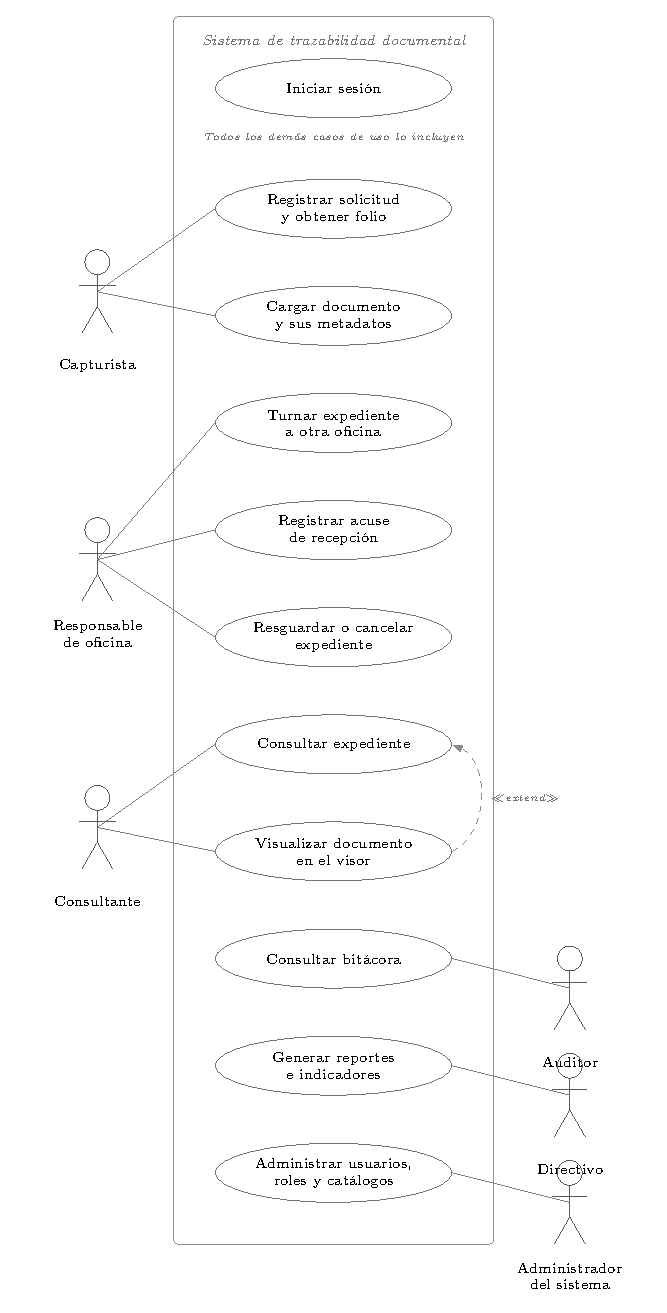
\includegraphics[height=0.80\textheight]{img/casos_uso.pdf}
  \caption{Diagrama general de casos de uso del sistema. Todos los casos de uso incluyen el inicio de sesión; la visualización en el visor extiende la consulta del expediente.}
  \label{fig:casos_uso}
\end{figure}

Dos relaciones del diagrama merecen explicación. El inicio de sesión se incluye en todos los demás casos de uso, por lo que se indica mediante una nota y no mediante once flechas que harían ilegible la figura. La visualización del documento se modela como extensión de la consulta del expediente, y no como caso de uso independiente, porque solo ocurre cuando el expediente localizado tiene documento asociado y el perfil del usuario lo autoriza; si cualquiera de las dos condiciones falla, la consulta concluye sin extenderse.

La Tabla~\ref{tab:cu_registro} especifica el caso de uso principal, que es el que concentra la aportación del sistema. Los demás casos de uso siguen la misma estructura y se documentan en el manual técnico.

\begin{table}[H]
  \centering
  \small
  \renewcommand{\arraystretch}{1.3}
  \caption{Especificación del caso de uso CU-02, registro de solicitud y asignación de folio.}
  \label{tab:cu_registro}
  \begin{tabularx}{\textwidth}{@{}>{\raggedright\arraybackslash}p{2.9cm}>{\raggedright\arraybackslash}X@{}}
    \toprule
    \textbf{Identificador} & CU-02. Registrar solicitud y obtener folio \\
    \midrule
    \textbf{Actor principal} & Capturista \\
    \textbf{Requerimientos} & RF-04, RF-05, RF-06, RF-15 \\
    \textbf{Objetivo específico} & Quinto objetivo: desarrollar los módulos del sistema \\
    \textbf{Precondición} & El usuario tiene sesión iniciada y está adscrito a una oficina activa \\
    \textbf{Flujo normal} &
      1. El capturista elige el tipo documental. \newline
      2. El sistema despliega los campos de metadato que el catálogo exige para ese tipo. \newline
      3. El capturista captura los metadatos y adjunta el archivo. \newline
      4. El sistema valida los metadatos obligatorios y el formato y tamaño del archivo. \newline
      5. El sistema asigna el folio dentro de una transacción con bloqueo de la fila del contador. \newline
      6. El sistema calcula la huella del archivo y lo guarda fuera de la raíz pública. \newline
      7. El sistema asienta el alta en la bitácora y muestra el acuse con el folio. \\
    \textbf{Flujos alternos} &
      4a. Falta un metadato obligatorio: el sistema señala el campo y no asigna folio. \newline
      4b. El archivo excede el tamaño o su firma binaria no corresponde a un formato admitido: el sistema lo rechaza y conserva los metadatos capturados. \newline
      5a. La transacción falla: se revierte por completo y no se consume consecutivo. \\
    \textbf{Postcondición} & Existe un expediente en estado \texttt{con\_documento}, con folio irrepetible, documento asociado con su huella y tres asientos en la bitácora \\
    \bottomrule
  \end{tabularx}
\end{table}


\subsection{Diagramas de base de datos} \label{sec:diagramas_bd} % audit:req=diagrama_bd

\begin{guia}[Guía: Diagramas de base de datos]
\textbf{Debe incluir:} el diagrama entidad-relación (o el modelo relacional / de documentos) y el
\textbf{diccionario de datos} (tabla por entidad: campo, tipo, restricciones, descripción).

\textbf{Debe responder:} ¿qué entidades y relaciones hay y por qué? ¿qué gestor de base de datos se usó y por qué? ¿está
normalizado? ¿cómo se protege la información (respaldos, permisos, datos personales)?

\textbf{Mínimo:} 1 diagrama (figura) con explicación.
\end{guia}

La Figura~\ref{fig:modelo_datos} presenta el modelo relacional implementado. Se organiza en tres bloques. Los \emph{catálogos} guardan lo que el área técnica administra sin tocar el código: oficinas, roles, usuarios, tipos documentales y los campos de metadato que cada tipo exige. El \emph{núcleo documental} guarda el expediente, sus valores de metadato, sus versiones de documento y el contador del que nace el folio. La \emph{trazabilidad} guarda los movimientos y la bitácora.

\begin{figure}[H]
  \centering
  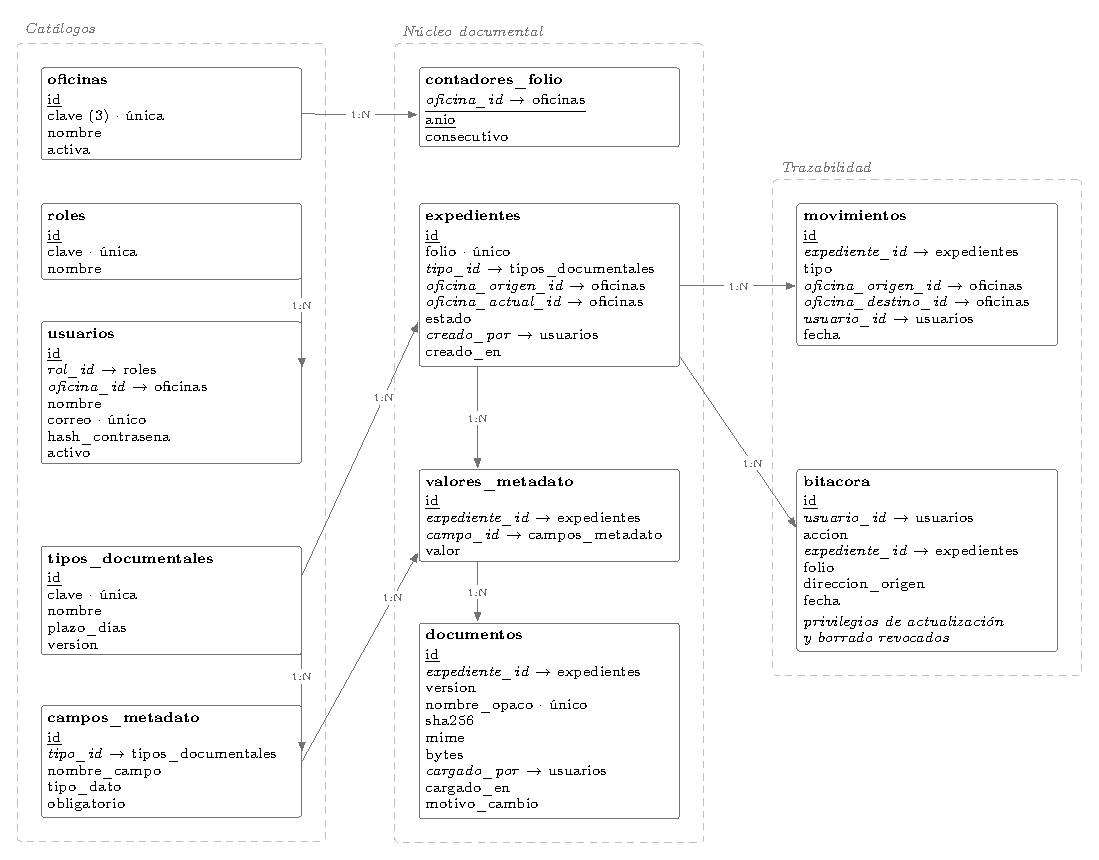
\includegraphics[width=\textwidth]{img/modelo_datos.pdf}
  \caption{Modelo relacional del sistema. Las llaves primarias aparecen subrayadas y las foráneas en cursiva con la tabla referida.}
  \label{fig:modelo_datos}
\end{figure}

El gestor es MariaDB con motor InnoDB. La elección respondió a tres condiciones: el Instituto ya lo opera, lo que evita introducir una tecnología más al área técnica; soporta transacciones con bloqueo de fila, sin las cuales el folio único no sería posible; y no implica costo de licenciamiento. El esquema está normalizado hasta la tercera forma normal: los metadatos no se guardan como columnas fijas del expediente sino en \texttt{valores\_metadato}, lo que elimina la dependencia entre el tipo documental y la estructura de la tabla, y permite agregar un tipo nuevo sin alterar el esquema.

Tres decisiones del modelo merecen justificarse. La primera es que \texttt{contadores\_folio} tenga llave primaria compuesta por oficina y año: así el consecutivo es independiente por oficina y reinicia solo, sin un proceso de cierre anual. La segunda es que \texttt{documentos} guarde versiones en lugar de sobrescribir: la sustitución inserta una fila nueva con su motivo y conserva la anterior, lo que atiende el punto de pérdida de trazabilidad por sustitución sin versionado. La tercera es que el archivo no se guarde en la base, sino su referencia y su huella; la base conserva solo la referencia y la huella, y no el contenido del archivo.

La Tabla~\ref{tab:diccionario} presenta el diccionario de datos de las dos tablas centrales. El diccionario completo de las once tablas se entrega en el manual técnico.

\begin{table}[H]
  \centering
  \small
  \renewcommand{\arraystretch}{1.25}
  \caption{Diccionario de datos de las tablas \texttt{expedientes} y \texttt{bitacora}.}
  \label{tab:diccionario}
  \begin{tabularx}{\textwidth}{@{}>{\raggedright\arraybackslash}p{3.6cm}>{\raggedright\arraybackslash}p{2.3cm}>{\raggedright\arraybackslash}p{2.5cm}>{\raggedright\arraybackslash}X@{}}
    \toprule
    \textbf{Campo} & \textbf{Tipo} & \textbf{Restricciones} & \textbf{Descripción} \\
    \midrule
    \multicolumn{4}{@{}l}{\textit{Tabla} \texttt{expedientes}} \\
    \addlinespace[2pt]
    \texttt{id} & BIGINT & PK, autoincremental & Identificador interno \\
    \texttt{folio} & CHAR(22) & Único, no nulo & Folio institucional con la plantilla \texttt{IRCT-OOO-AAAA-NNNNNN} \\
    \texttt{tipo\_id} & BIGINT & FK, no nulo & Tipo documental del catálogo \\
    \texttt{oficina\_origen\_id} & BIGINT & FK, no nulo & Oficina que registró el expediente \\
    \texttt{oficina\_actual\_id} & BIGINT & FK, no nulo & Oficina que lo tiene en su poder \\
    \texttt{estado} & ENUM & No nulo & \texttt{registrado}, \texttt{con\_documento}, \texttt{en\_tramite}, \texttt{recibido}, \texttt{resguardado} o \texttt{cancelado} \\
    \texttt{creado\_por} & BIGINT & FK, no nulo & Usuario que lo registró \\
    \texttt{creado\_en} & DATETIME & No nulo & Fecha y hora del registro \\
    \addlinespace[4pt]
    \multicolumn{4}{@{}l}{\textit{Tabla} \texttt{bitacora}} \\
    \addlinespace[2pt]
    \texttt{id} & BIGINT & PK, autoincremental & Identificador del asiento \\
    \texttt{usuario\_id} & BIGINT & FK, no nulo & Quien ejecutó la acción \\
    \texttt{accion} & VARCHAR(40) & No nulo, indexado & Acción asentada \\
    \texttt{expediente\_id} & BIGINT & FK, nulo permitido & Expediente afectado, nulo en accesos sin expediente \\
    \texttt{folio} & CHAR(22) & Nulo permitido & Folio al momento del asiento, conservado aunque el expediente cambie \\
    \texttt{direccion\_origen} & VARCHAR(45) & No nulo & Dirección de red desde la que se operó \\
    \texttt{fecha} & DATETIME(3) & No nulo, indexado & Marca temporal con precisión de milisegundo \\
    \bottomrule
  \end{tabularx}
\end{table}

La protección de la información descansa en tres mecanismos. El primero es el privilegio: la cuenta con la que se conecta la aplicación tiene revocados los permisos de actualización y borrado sobre \texttt{bitacora}, de modo que la inmutabilidad no depende del código. El segundo es el respaldo diario de la base y del acervo, con restauración probada antes de la liberación. El tercero atiende la protección de datos personales que impone la ley aplicable \cite{lgpdppso2017}: los nombres de las partes que aparecen en los metadatos solo son visibles para los perfiles con ámbito sobre ese expediente, y las exportaciones de reportes agregados no incluyen datos personales, sino conteos.


\subsection{Diagramas de actividades} \label{sec:diagramas_actividades} % audit:req=diagrama_actividades

\begin{guia}[Guía: Diagramas de actividades]
\textbf{Debe incluir:} el flujo de los procesos clave del sistema (con carriles o \emph{swimlanes} por actor cuando hay
varios participantes), con inicio, decisiones, acciones y fin.

\textbf{Debe responder:} ¿cuál es el flujo de cada proceso importante? ¿qué pasa en los casos de error? ¿corresponde a
algún caso de uso?

\textbf{Mínimo:} 1 diagrama (figura) con explicación.
\end{guia}

La Figura~\ref{fig:actividades} presenta el flujo del proceso documental completo, desde la captura hasta el cierre del expediente, repartido en tres carriles: el capturista, el sistema y el responsable de la oficina destino. El diagrama corresponde a los casos de uso CU-02 a CU-05 y hace visible la división de responsabilidades que la propuesta enuncia: las personas deciden y capturan, el sistema valida, numera, guarda y deja constancia.

\begin{figure}[H]
  \centering
  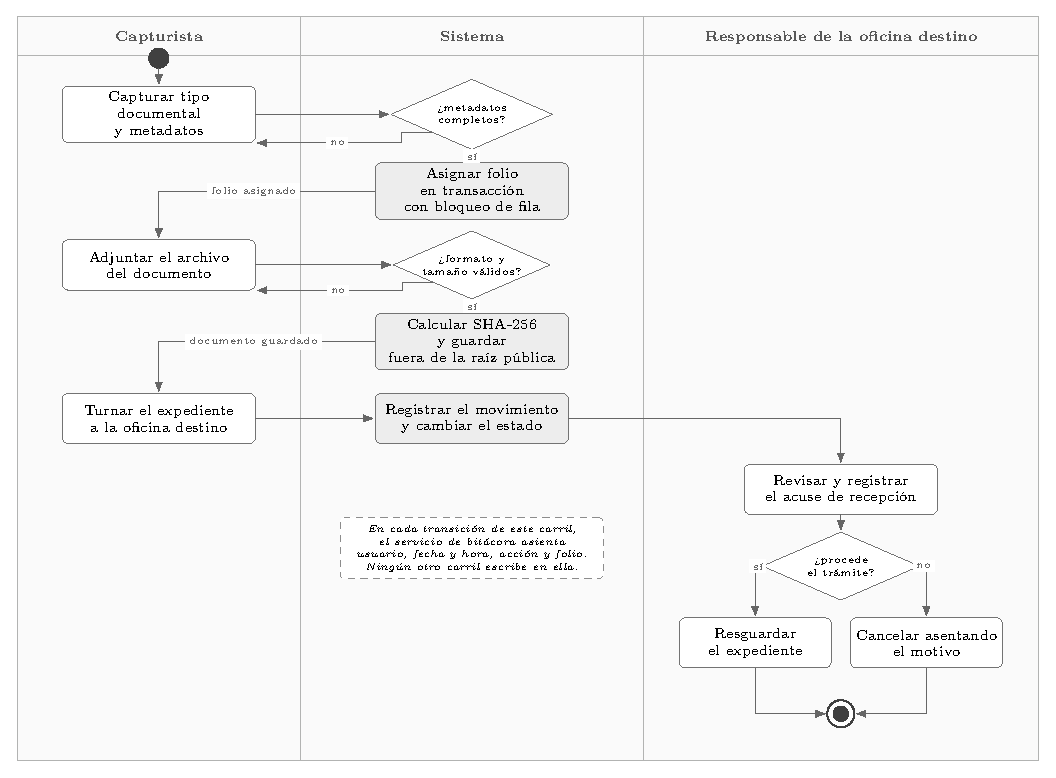
\includegraphics[width=\textwidth]{img/actividades.pdf}
  \caption{Diagrama de actividades del proceso documental, con carriles por participante. El carril del sistema concentra las validaciones y los asientos en la bitácora.}
  \label{fig:actividades}
\end{figure}

El flujo tiene dos puntos de decisión en el carril del sistema y uno en el del responsable. Los dos primeros son controles de admisión: si los metadatos obligatorios del tipo documental están incompletos, el expediente no nace y no se consume folio; si el archivo no corresponde a un formato admitido o excede el tamaño, se rechaza conservando los metadatos ya capturados, de modo que el capturista no tenga que volver a escribirlos. Esta diferencia no es menor: el primer rechazo ocurre antes de asignar folio, y el segundo después, cuando el expediente ya existe en estado \texttt{registrado}.

El tercer punto de decisión corresponde a la resolución del trámite. El camino afirmativo conduce al resguardo del expediente; el negativo, a su cancelación con motivo asentado. La cancelación no borra nada: cambia el estado y agrega un asiento, de modo que un expediente cancelado conserva íntegro su historial y puede auditarse igual que uno resguardado.

Conviene señalar qué no aparece en el diagrama y por qué. No hay un carril para la bitácora, pese a ser el componente central del sistema, porque la bitácora no decide ni ramifica: se escribe en cada transición del carril del sistema, sin excepción y sin intervención humana. Representarla como un participante más sugeriría que alguien puede omitirla, que es justamente lo que el diseño impide. Por eso aparece como nota transversal al carril del sistema.


\subsection{Diagramas de secuencia} \label{sec:diagramas_secuencia} % audit:req=diagrama_secuencia

\begin{guia}[Guía: Diagramas de secuencia]
\textbf{Debe incluir:} la interacción entre los componentes (usuario, interfaz, servidor, base de datos, servicios
externos) para los casos de uso críticos, con los mensajes en orden temporal.

\textbf{Debe responder:} ¿qué componentes intervienen y en qué orden se comunican? ¿qué mensajes se envían y qué se
responde? ¿dónde se validan los datos?

\textbf{Mínimo:} 1 diagrama (figura) con explicación.
\end{guia}

La Figura~\ref{fig:secuencia} detalla la interacción entre componentes para el caso de uso CU-02, que es el crítico del sistema porque en él se asigna el folio. Participan seis objetos: el capturista, el controlador de solicitudes, los tres servicios de dominio y la base de datos.

\begin{figure}[H]
  \centering
  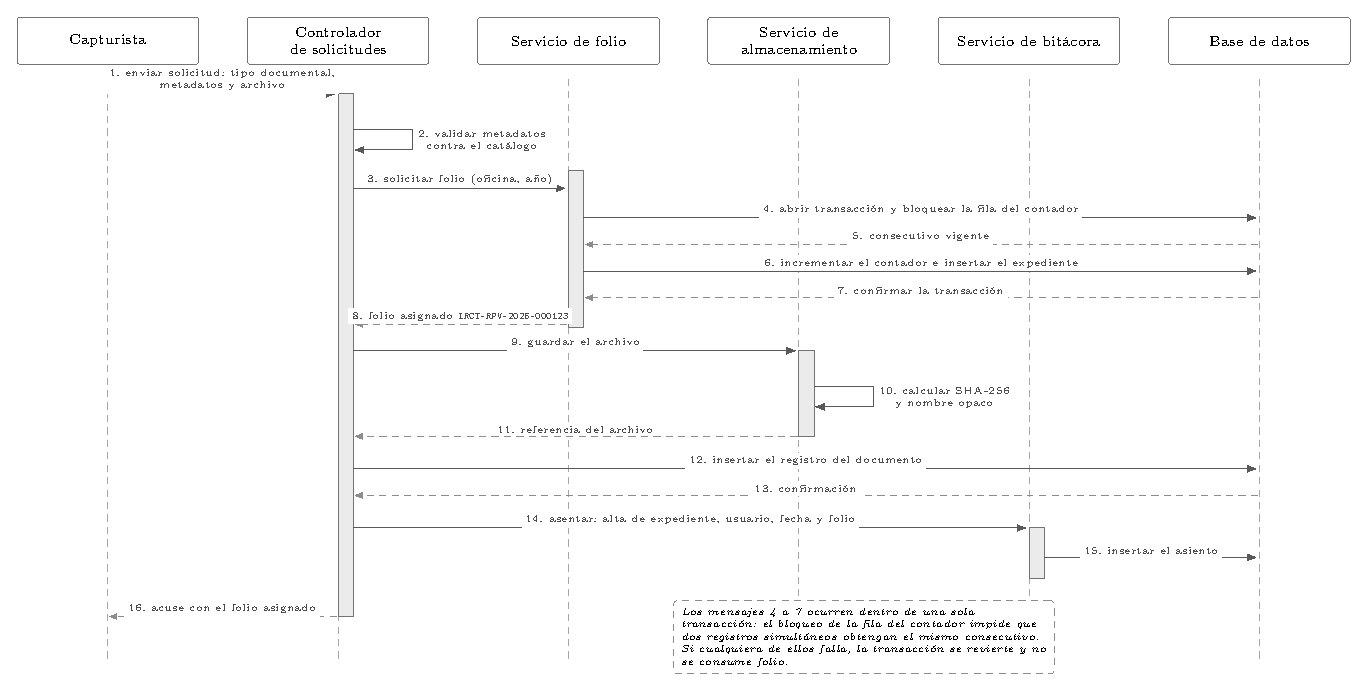
\includegraphics[width=\textwidth]{img/secuencia.pdf}
  \caption{Diagrama de secuencia del registro de una solicitud con asignación de folio. Los mensajes 4 a 7 transcurren dentro de una sola transacción.}
  \label{fig:secuencia}
\end{figure}

El orden de los mensajes responde a una regla de diseño: nada irreversible ocurre antes de que todo lo reversible haya sido validado. Por eso el mensaje 2, la validación de los metadatos contra el catálogo, precede a la solicitud del folio. Si se invirtiera el orden, un formulario incompleto consumiría un consecutivo que después quedaría como hueco en la secuencia, y la prueba de unicidad fallaría no por duplicados sino por discontinuidad.

La validación ocurre en tres lugares distintos y conviene no confundirlos. La validación de los metadatos obligatorios se hace en el controlador, contra el catálogo vigente (mensaje 2). La validación del formato y el tamaño del archivo se hace en el servicio de almacenamiento, comprobando la firma binaria y no la extensión (mensaje 10). Y la validación del permiso se hace antes de todo lo anterior, en la política de autorización, que no aparece en el diagrama porque interviene en el enrutamiento, antes de que el controlador reciba la petición. Ninguna de las tres ocurre en el navegador: la interfaz señala los errores por comodidad del usuario, pero la decisión siempre se toma en el servidor, conforme a RNF-02.

Los mensajes 4 a 7 constituyen el núcleo de la garantía de unicidad. El servicio de folio abre la transacción y bloquea en exclusiva la fila del contador que corresponde a la oficina y al año; cualquier otra petición que intente obtener folio para esa misma combinación espera a que la transacción concluya. Dentro de ese bloqueo se lee el consecutivo vigente, se incrementa y se inserta el expediente. Si cualquiera de los tres pasos falla, la transacción se revierte completa y el contador queda como estaba, de modo que un error no consume folio ni deja huecos.

El Algoritmo~\ref{alg:folio} expresa ese núcleo en pseudocódigo. Dos detalles merecen atención. El primero es la línea 3: si la oficina no tiene aún contador para el año en curso, la fila se crea y se bloquea dentro de la misma transacción, de modo que el primer registro del año no constituya una ventana sin protección. El segundo es que la restricción de unicidad sobre la terna oficina, año y consecutivo actúa como segunda barrera: si por un error de programación dos transacciones llegaran a componer el mismo folio, el motor rechazaría la segunda inserción y la transacción se revertiría.

\begin{algorithm}[H]
\caption{Asignación del folio institucional}
\label{alg:folio}
\begin{algorithmic}[1]
\Require oficina $o$, año $a$
\Ensure folio único con la plantilla \texttt{IRCT-OOO-AAAA-NNNNNN}
\State iniciar transacción
\State $c \gets$ seleccionar consecutivo de \texttt{contadores\_folio} para $(o,a)$ \textbf{para actualizar}
\If{no existe la fila}
  \State insertar $(o, a, 0)$ y bloquearla
  \State $c \gets 0$
\EndIf
\State $c \gets c + 1$
\State actualizar \texttt{contadores\_folio} con $c$ para $(o,a)$
\State $f \gets$ concatenar \texttt{IRCT}, clave de $o$, $a$ y $c$ rellenado a seis dígitos
\State insertar expediente con folio $f$
\If{alguna operación falló}
  \State revertir transacción
  \State \Return error, sin consumir consecutivo
\EndIf
\State confirmar transacción
\State \Return $f$
\end{algorithmic}
\end{algorithm}

Por último, el asiento en bitácora (mensaje 14) ocurre después de que el documento quedó guardado, no antes. La razón es que la bitácora debe consignar hechos consumados: un asiento que registrara una carga que después falló convertiría la bitácora en una relación de intenciones y no de hechos, y el control estadístico derivado de ella perdería el sustento que justifica llamarla única fuente.


\subsection{Resultado final: pantallas del sistema} \label{sec:pantallas} % audit:req=pantallas

\begin{guia}[Guía: Resultado final -- pantallas del sistema con su explicación]
\textbf{Debe incluir:} capturas de las pantallas principales del sistema funcionando, cada una con su explicación.

\textbf{Para cada pantalla responde:} ¿para qué sirve? ¿quién la usa? ¿qué casos de uso y objetivos específicos
atiende? ¿qué datos muestra o captura y cómo se valida?

\textbf{Reglas:} figuras numeradas con \verb|\caption| y \verb|\label|; sin datos personales ni confidenciales reales
(usa datos de prueba); capturas legibles. Si hay versión móvil o de escritorio, inclúyela.

\textbf{Mínimo:} 150 palabras de explicación y al menos una figura.
\end{guia}

Esta subsección presenta las diez pantallas principales del sistema en operación. Las capturas se tomaron del entorno de pruebas el 20 de noviembre de 2026, con datos ficticios: los nombres de personas, las claves catastrales y los folios reales que aparecen no corresponden a ningún expediente del Instituto, conforme a la obligación de no exhibir datos personales de los titulares. Las fechas de vencimiento y los semáforos que se ven en las figuras son los que el sistema calcula para esa fecha de referencia con los plazos del catálogo, no valores ilustrativos. Se capturaron a mil píxeles de ancho de ventana —por encima del mínimo comprometido en RNF-06 y por debajo del escritorio habitual— para que el texto de la interfaz siga siendo legible al reducir la imagen al ancho de esta página. La interfaz emplea la paleta institucional del Gobierno del Estado de Tamaulipas y se organiza siempre igual: barra superior con la identificación del usuario, su rol y su oficina de adscripción; menú lateral con las opciones que su perfil habilita, apareciendo atenuadas las que no; y área de trabajo. Que el menú muestre las opciones no disponibles en lugar de ocultarlas es deliberado: el usuario comprende el alcance de su perfil y sabe a qué puede solicitar acceso.

\subsubsection*{Inicio de sesión}

La Figura~\ref{fig:pant_login} muestra el acceso al sistema. Captura credencial institucional y contraseña, y advierte, antes de cualquier intento, que la cuenta se bloquea a los cinco fallos consecutivos conforme a RF-01; el mensaje de error nunca revela si fue el usuario o la contraseña lo que no correspondía, para no confirmar la existencia de una cuenta. La contraseña viaja cifrada por TLS y se contrasta contra una derivación con sal, nunca contra un valor almacenado en claro. El aviso inferior cumple una función que no es decorativa: informa al usuario, antes de entrar, que sus acciones quedarán asentadas en la bitácora y que la sesión se cierra sola a los veinte minutos de inactividad, conforme a RF-03, porque los equipos de ventanilla son compartidos. Es a la vez un requisito de transparencia y un disuasor eficaz.

\begin{figure}[H]
  \centering
  
\includegraphics[width=\textwidth,height=0.78\textheight,keepaspectratio]{img/pantalla-acceso.png}
  \caption{Pantalla de inicio de sesión. Atiende el caso de uso CU-01 y el requerimiento RF-01.}
  \label{fig:pant_login}
\end{figure}

\subsubsection*{Bandeja de expedientes}

La Figura~\ref{fig:pant_bandeja} es la pantalla de trabajo cotidiano. Lista los expedientes del ámbito del usuario —y solo esos: el alcance de oficina se aplica en la consulta, no en la presentación, de modo que un expediente de otra oficina no llega siquiera al navegador— con filtros por folio, tipo documental, estado y rango de fechas. Cada renglón muestra el estado mediante una etiqueta y el plazo mediante un semáforo de tres niveles acompañado de los días hábiles que restan: verde cuando queda margen, ámbar cuando se ha consumido el ochenta por ciento del plazo y rojo cuando venció, conforme a RF-13. Los expedientes ya cerrados —resguardados o cancelados— no muestran semáforo, porque dejarlos en rojo inflaría el indicador de vencidos del tablero con trabajo ya concluido. La leyenda al pie recuerda el criterio de ámbito, para que nadie interprete el conteo como el total institucional.

\begin{figure}[H]
  \centering
  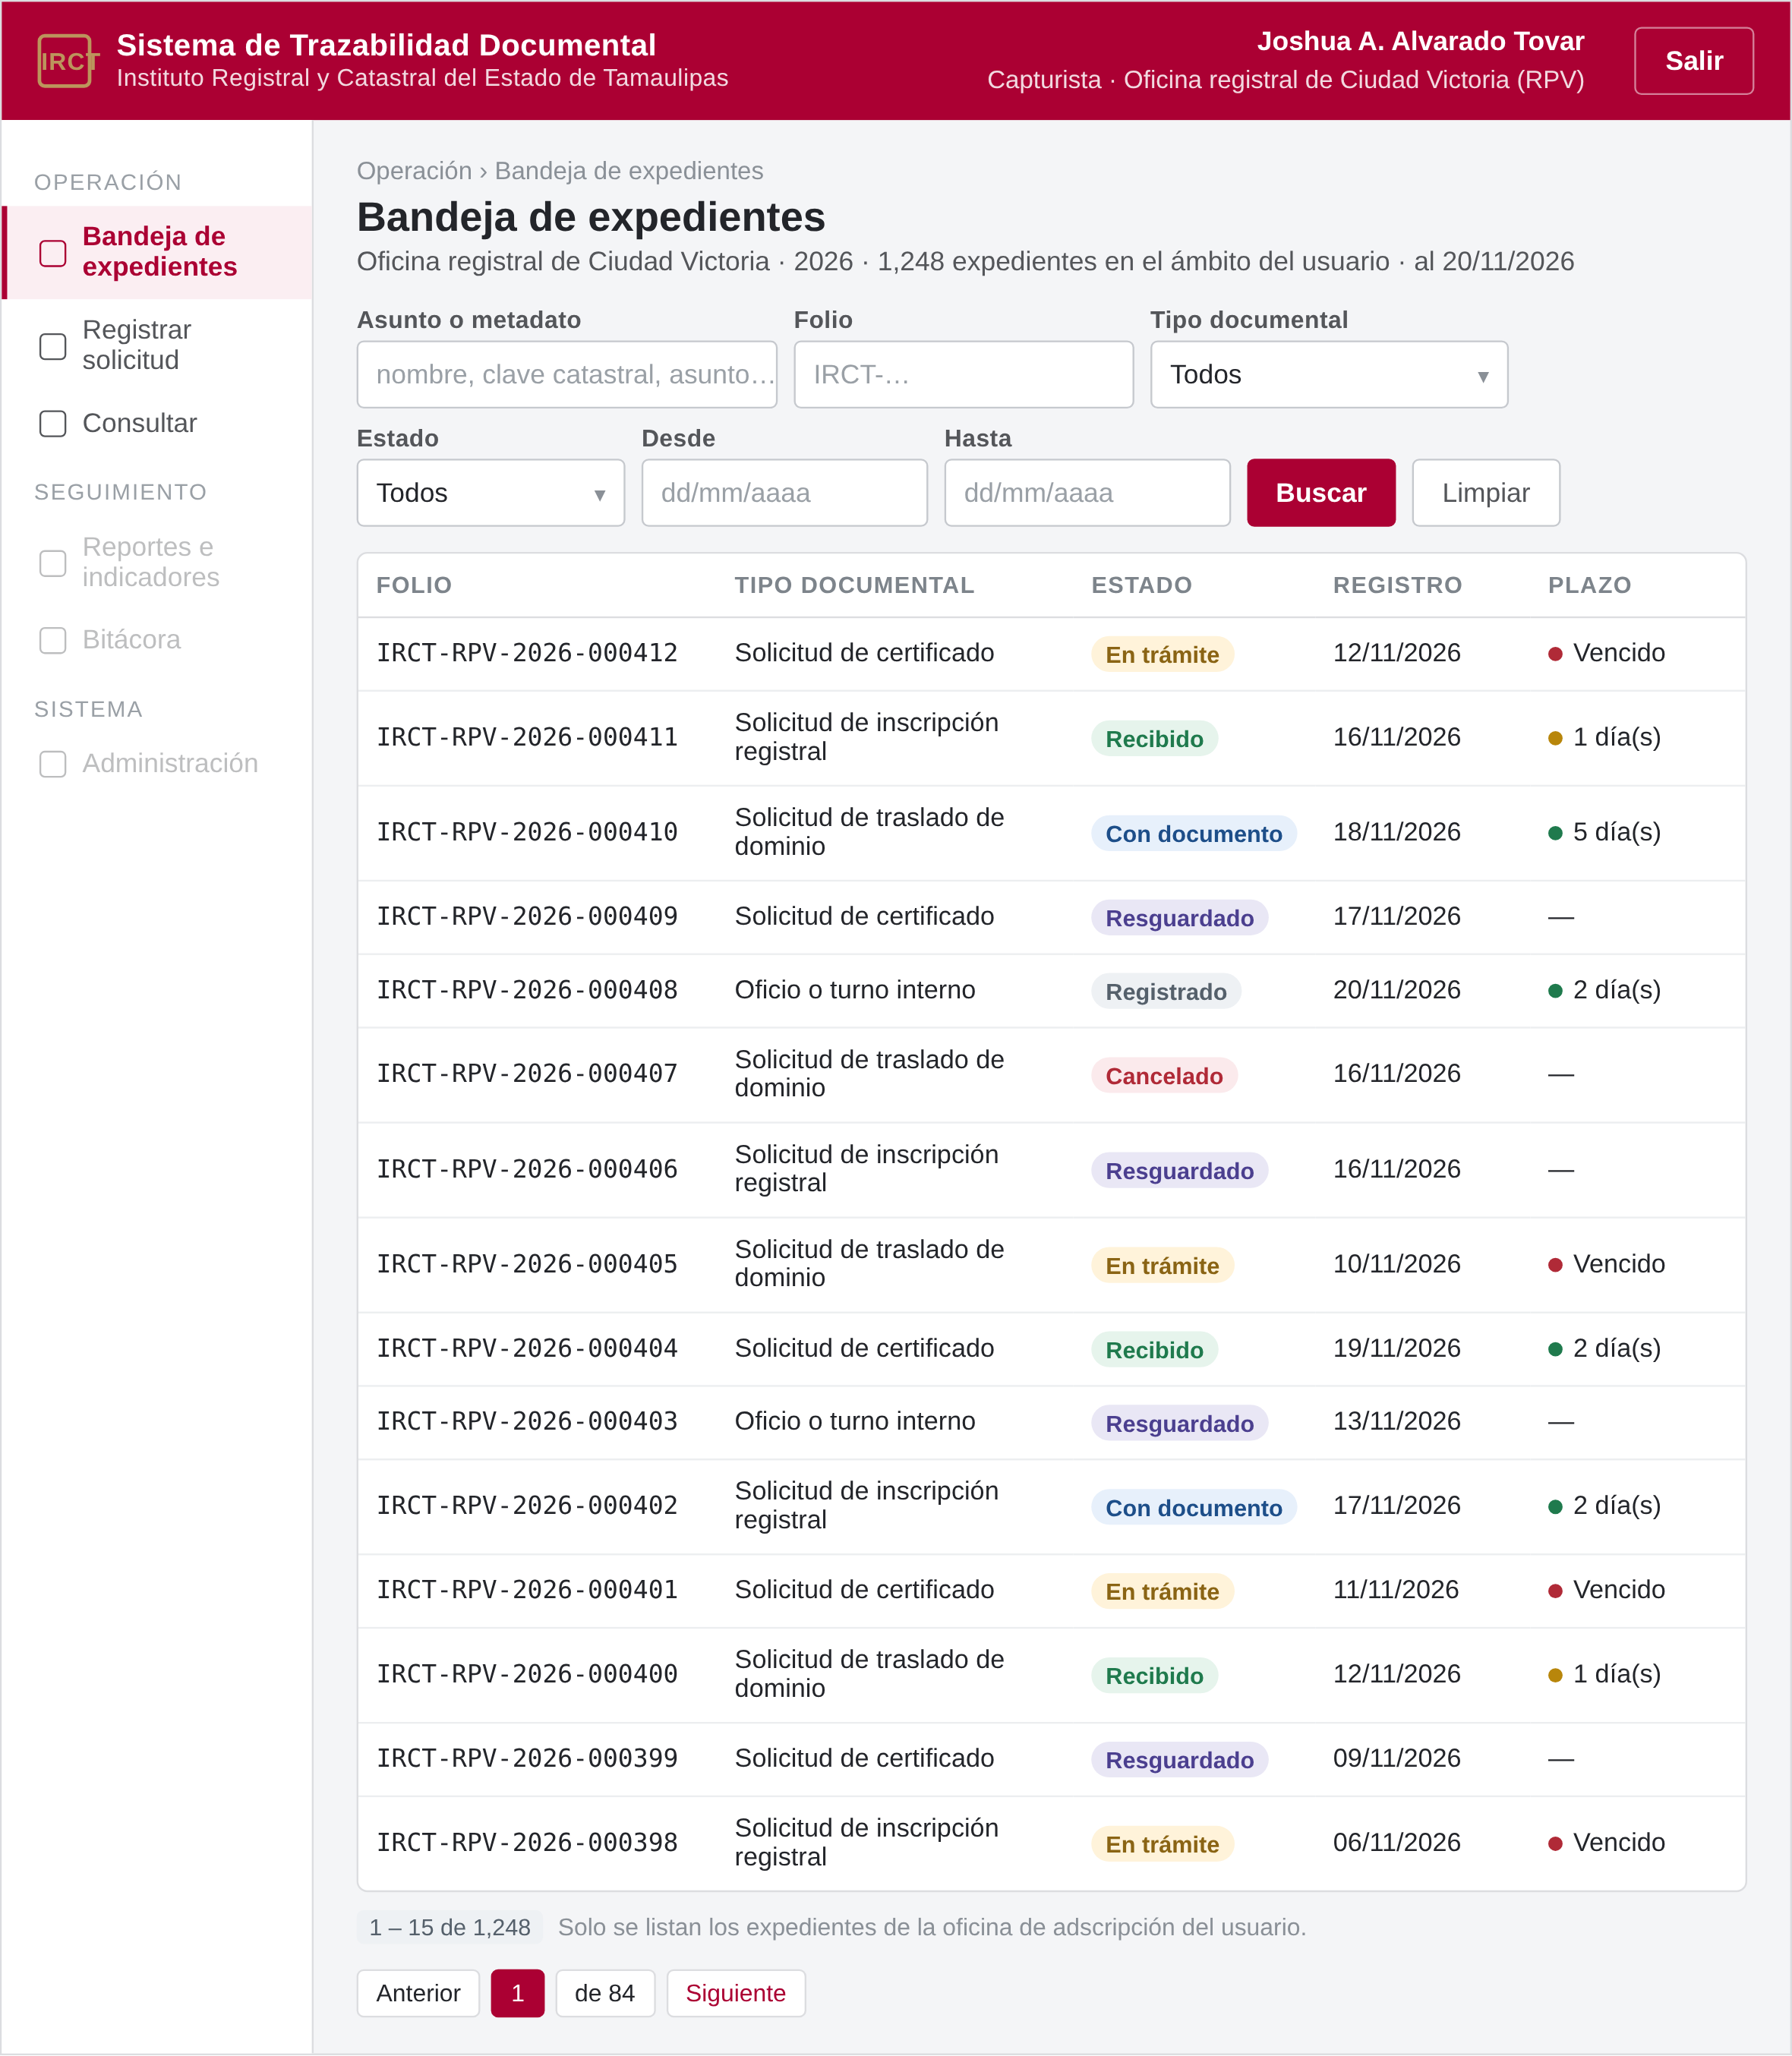
\includegraphics[width=\textwidth,height=0.78\textheight,keepaspectratio]{img/pantalla-bandeja.png}
  \caption{Bandeja de expedientes del capturista, con filtros y semáforo de plazos. Atiende CU-06 y los requerimientos RF-02, RF-09 y RF-13.}
  \label{fig:pant_bandeja}
\end{figure}

\subsubsection*{Registro de solicitud}

La Figura~\ref{fig:pant_registro} muestra el formulario de alta. Los campos de metadato no son fijos: se generan a partir del catálogo de tipos documentales, de modo que elegir «solicitud de traslado de dominio» despliega clave catastral, folio real, enajenante, adquirente y valor de la operación, mientras que otro tipo desplegaría otros campos. El panel derecho desglosa la plantilla del folio componente por componente y explica, en el propio punto de uso, por qué el consecutivo no puede repetirse; también muestra el plazo aplicable y su fecha de vencimiento, calculada en días hábiles. El recuadro de carga indica los formatos y tamaños admitidos y advierte que el archivo se verifica contra su firma binaria, no contra su extensión.

\begin{figure}[H]
  \centering
  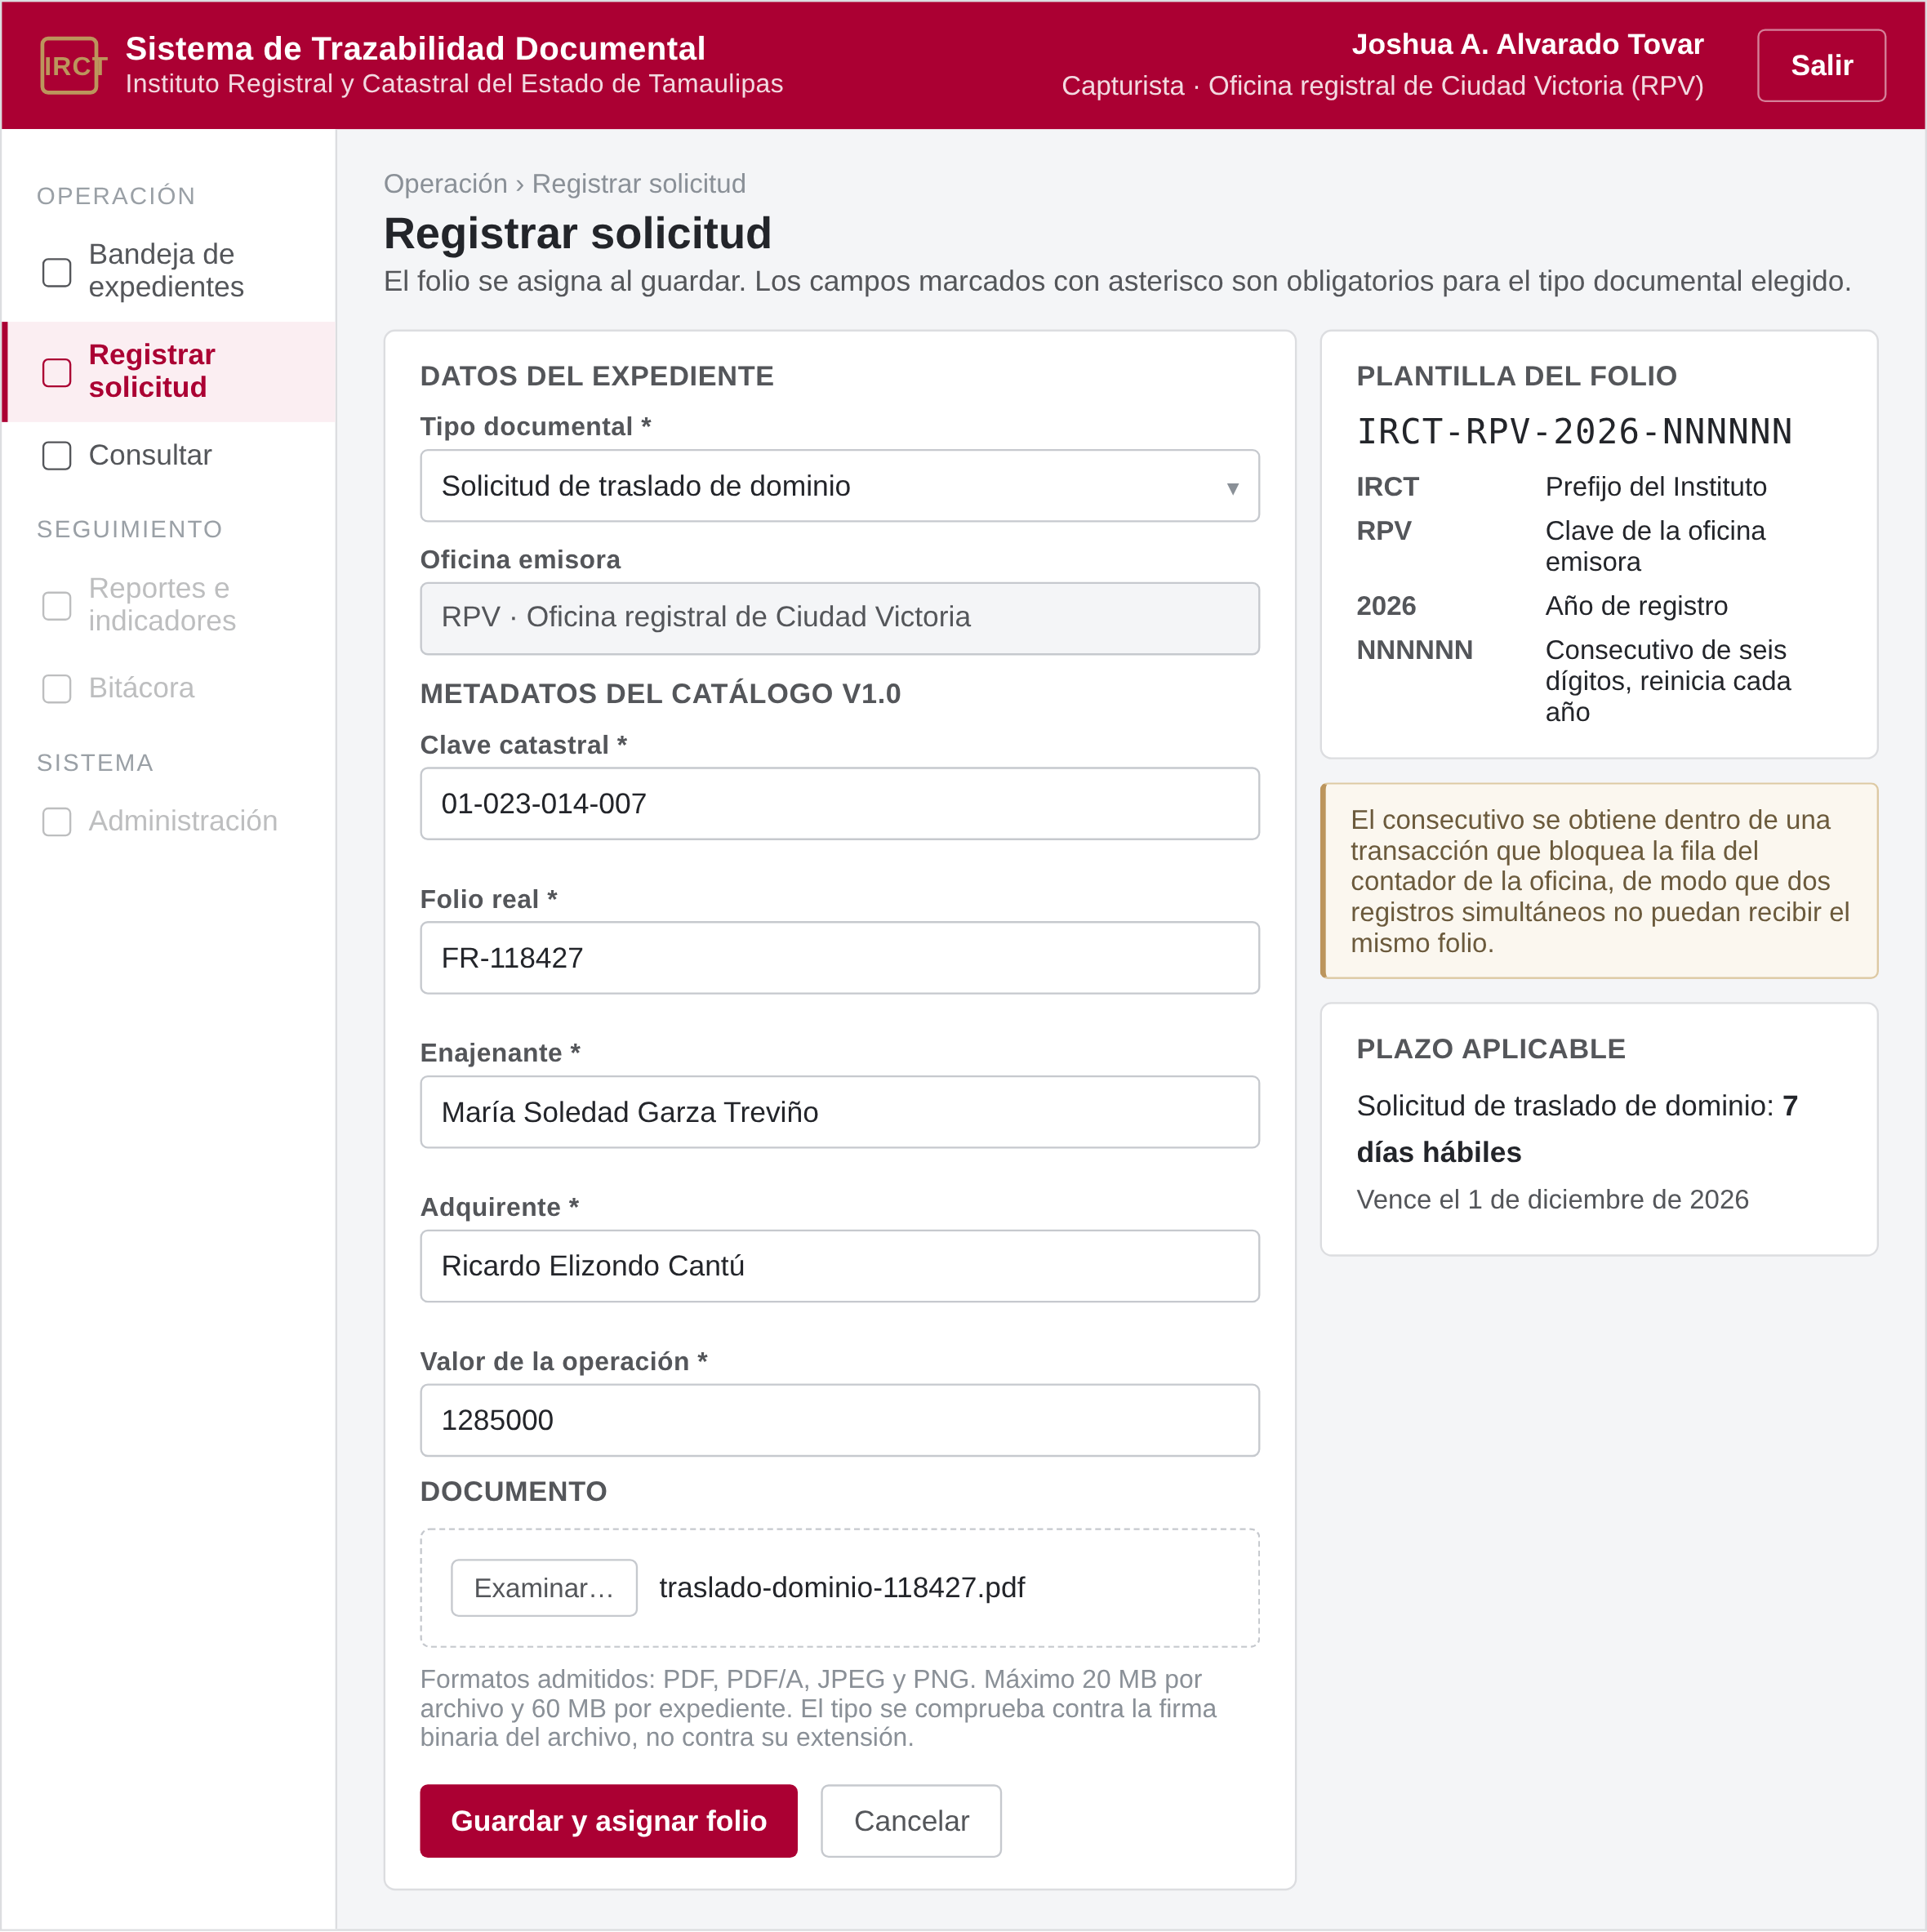
\includegraphics[width=\textwidth,height=0.78\textheight,keepaspectratio]{img/pantalla-registro.png}
  \caption{Formulario de registro de solicitud, con los metadatos que el catálogo exige para el tipo documental elegido. Atiende CU-02 y los requerimientos RF-04, RF-05 y RF-06.}
  \label{fig:pant_registro}
\end{figure}

\subsubsection*{Acuse de registro}

La Figura~\ref{fig:pant_acuse} presenta el acuse. Muestra el folio ya asignado, los metadatos capturados, el estado resultante y la huella SHA-256 del archivo, que es el dato con el que cualquiera puede verificar después que el documento no fue alterado. El panel derecho reproduce los tres asientos que la operación generó en la bitácora, con su hora exacta. Esa reproducción es importante para el argumento del sistema: el acuse no es un documento aparte que pudiera discrepar del registro, sino una vista de lo ya asentado.

\begin{figure}[H]
  \centering
  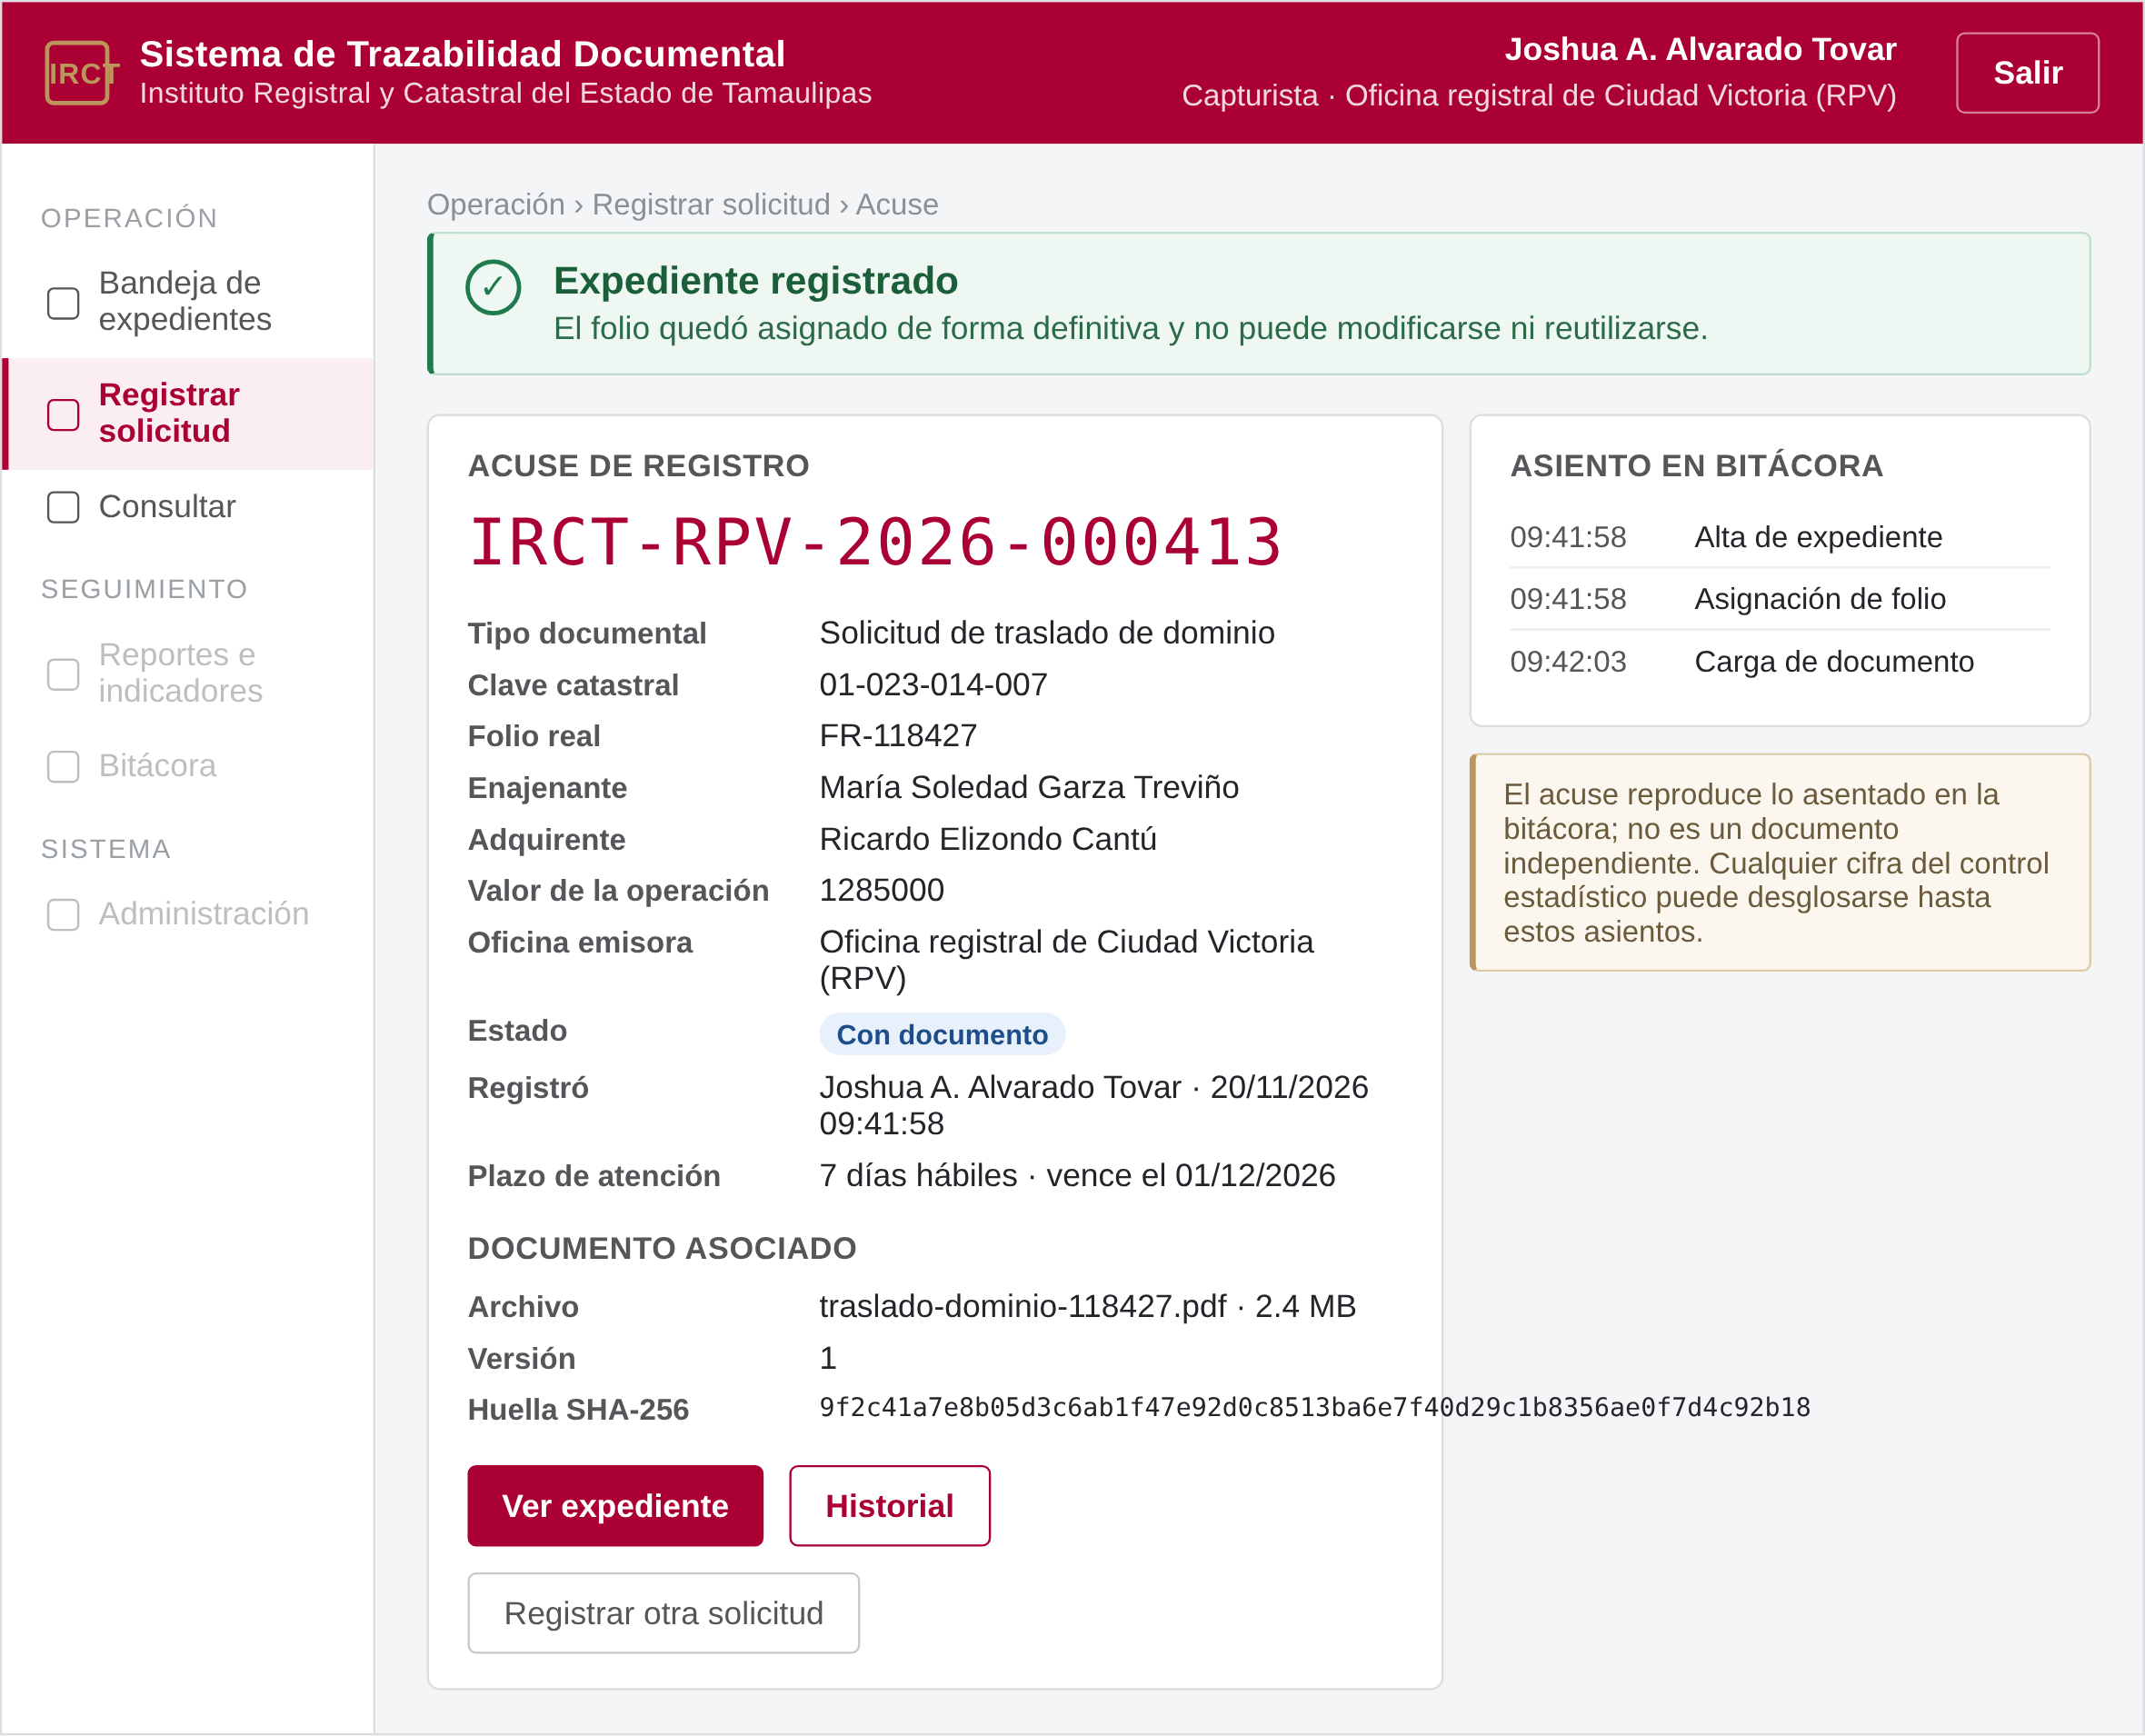
\includegraphics[width=\textwidth,height=0.78\textheight,keepaspectratio]{img/pantalla-acuse.png}
  \caption{Acuse emitido tras el registro, con el folio asignado y la huella del documento. Atiende CU-02 y los requerimientos RF-04, RF-06 y RF-15.}
  \label{fig:pant_acuse}
\end{figure}

\subsubsection*{Expediente y visor de documento}

La Figura~\ref{fig:pant_visor} muestra la consulta de un expediente. A la izquierda, los metadatos y el historial de movimientos, que cubre toda la vida del expediente y no solo su circulación: el alta con la asignación de folio, la carga del documento, su sustitución a la versión 2, el turnado y el acuse de la oficina receptora, cada uno con su hora y con el servidor público que lo ejecutó. A la derecha, el visor integrado. La captura corresponde a la sesión de un perfil de consultante adscrito a la oficina catastral, y el expediente se encuentra ya en la oficina registral por haber sido turnado: la oficina de origen conserva la visibilidad sobre lo que turnó, pues de otro modo perdería el rastro de sus propios asuntos en cuanto salieran de su escritorio. La barra del visor indica que la descarga no está autorizada para ese perfil: el documento se ve, pero el archivo no sale del sistema. El archivo se entrega por una ruta de la aplicación que verifica rol y oficina en cada petición, de modo que la dirección no es adivinable ni puede compartirse.

\begin{figure}[H]
  \centering
  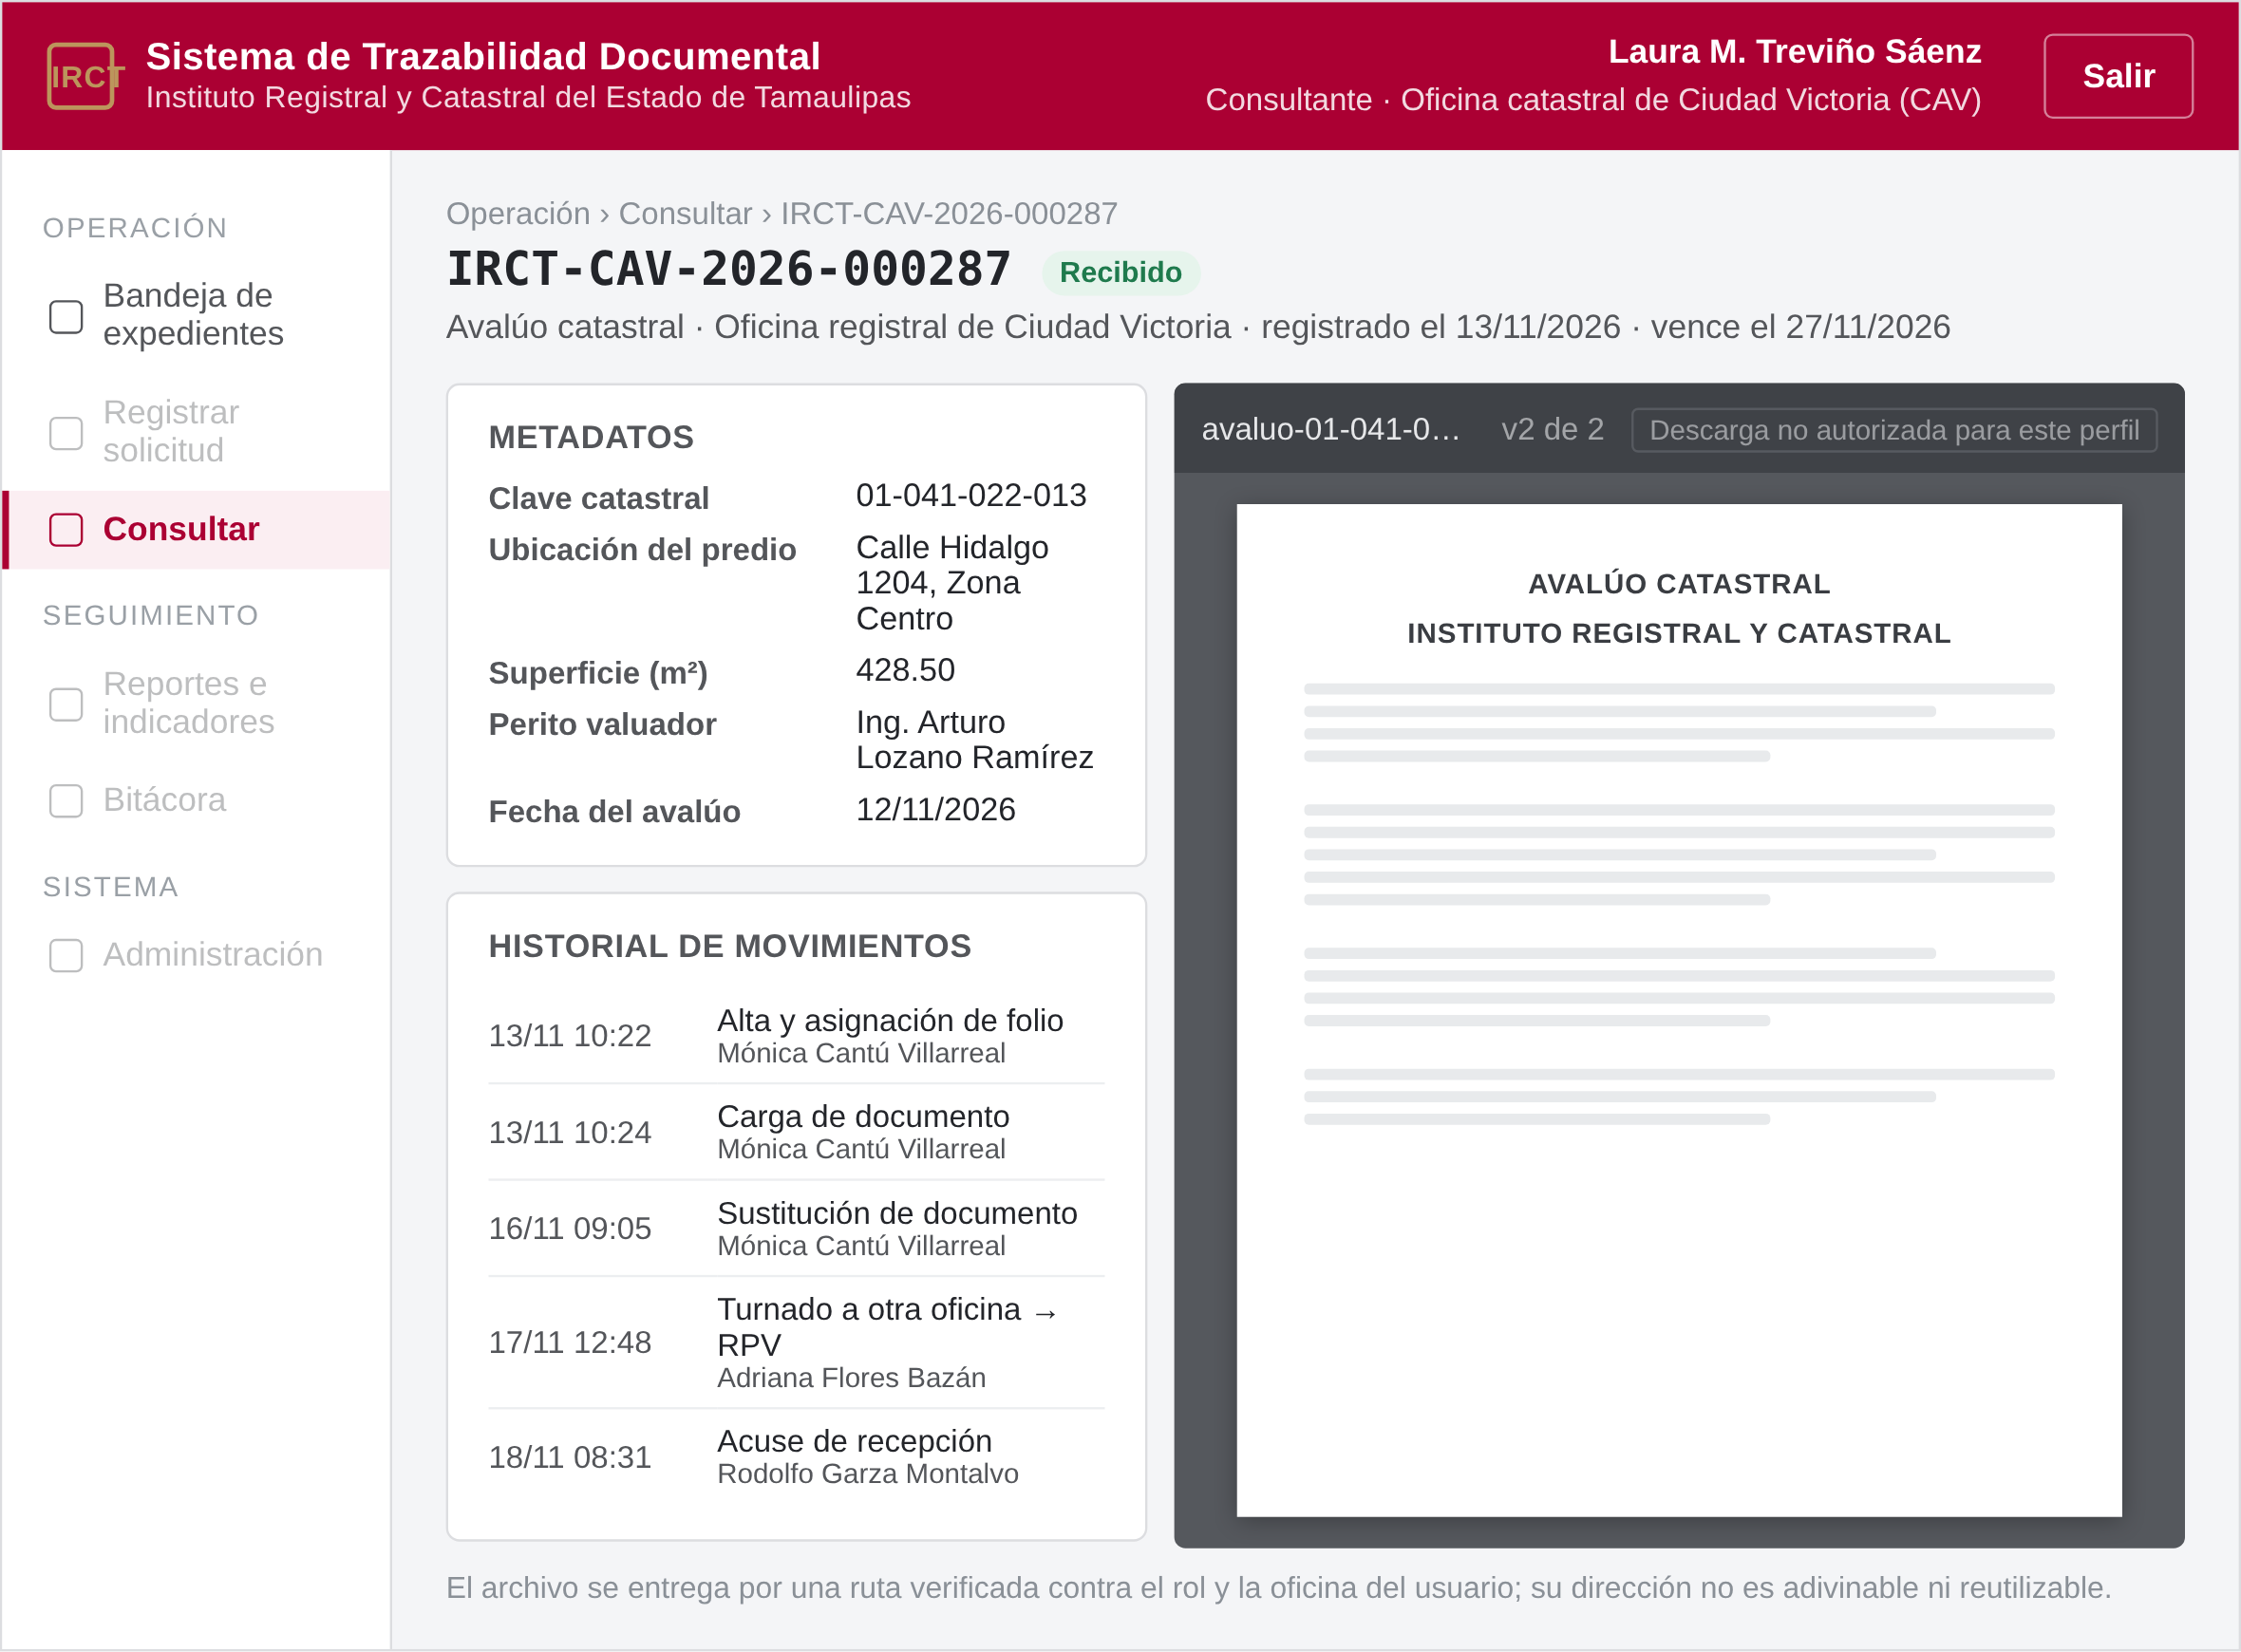
\includegraphics[width=\textwidth,height=0.78\textheight,keepaspectratio]{img/pantalla-visor.png}
  \caption{Consulta de expediente con el visor integrado, en la sesión de un consultante de la oficina catastral sobre un expediente que esa oficina ya turnó a la registral. Atiende CU-06 y CU-07 y los requerimientos RF-10 y RF-11.}
  \label{fig:pant_visor}
\end{figure}

\subsubsection*{Control estadístico}

La Figura~\ref{fig:pant_estadistico} presenta el control estadístico. Los cuatro indicadores superiores y las dos distribuciones se calculan a partir de los asientos de bitácora, sin contadores paralelos: la cifra y su evidencia son el mismo dato, que es lo que permite afirmar que lo reportado es comprobable. Los filtros cubren las cuatro dimensiones comprometidas en RF-12 —periodo, oficina, tipo documental y usuario—, y el tablero ofrece dos salidas: una hoja de cálculo y una versión imprimible que el navegador convierte a PDF. No se compone el PDF en el servidor de forma deliberada: una biblioteca de composición habría agregado una dependencia pesada que el área técnica del Instituto tendría que mantener y actualizar por seguridad, para producir un archivo que el navegador ya compone con fidelidad desde una hoja de estilo de impresión. Ambas salidas declaran siempre el periodo, los filtros aplicados, quién las generó y cuándo, para que un reporte impreso no pueda interpretarse fuera de contexto, y ambas dejan su propio asiento en la bitácora. La leyenda al pie enuncia la propiedad que verifica el cuarto criterio de aceptación.

\begin{figure}[H]
  \centering
  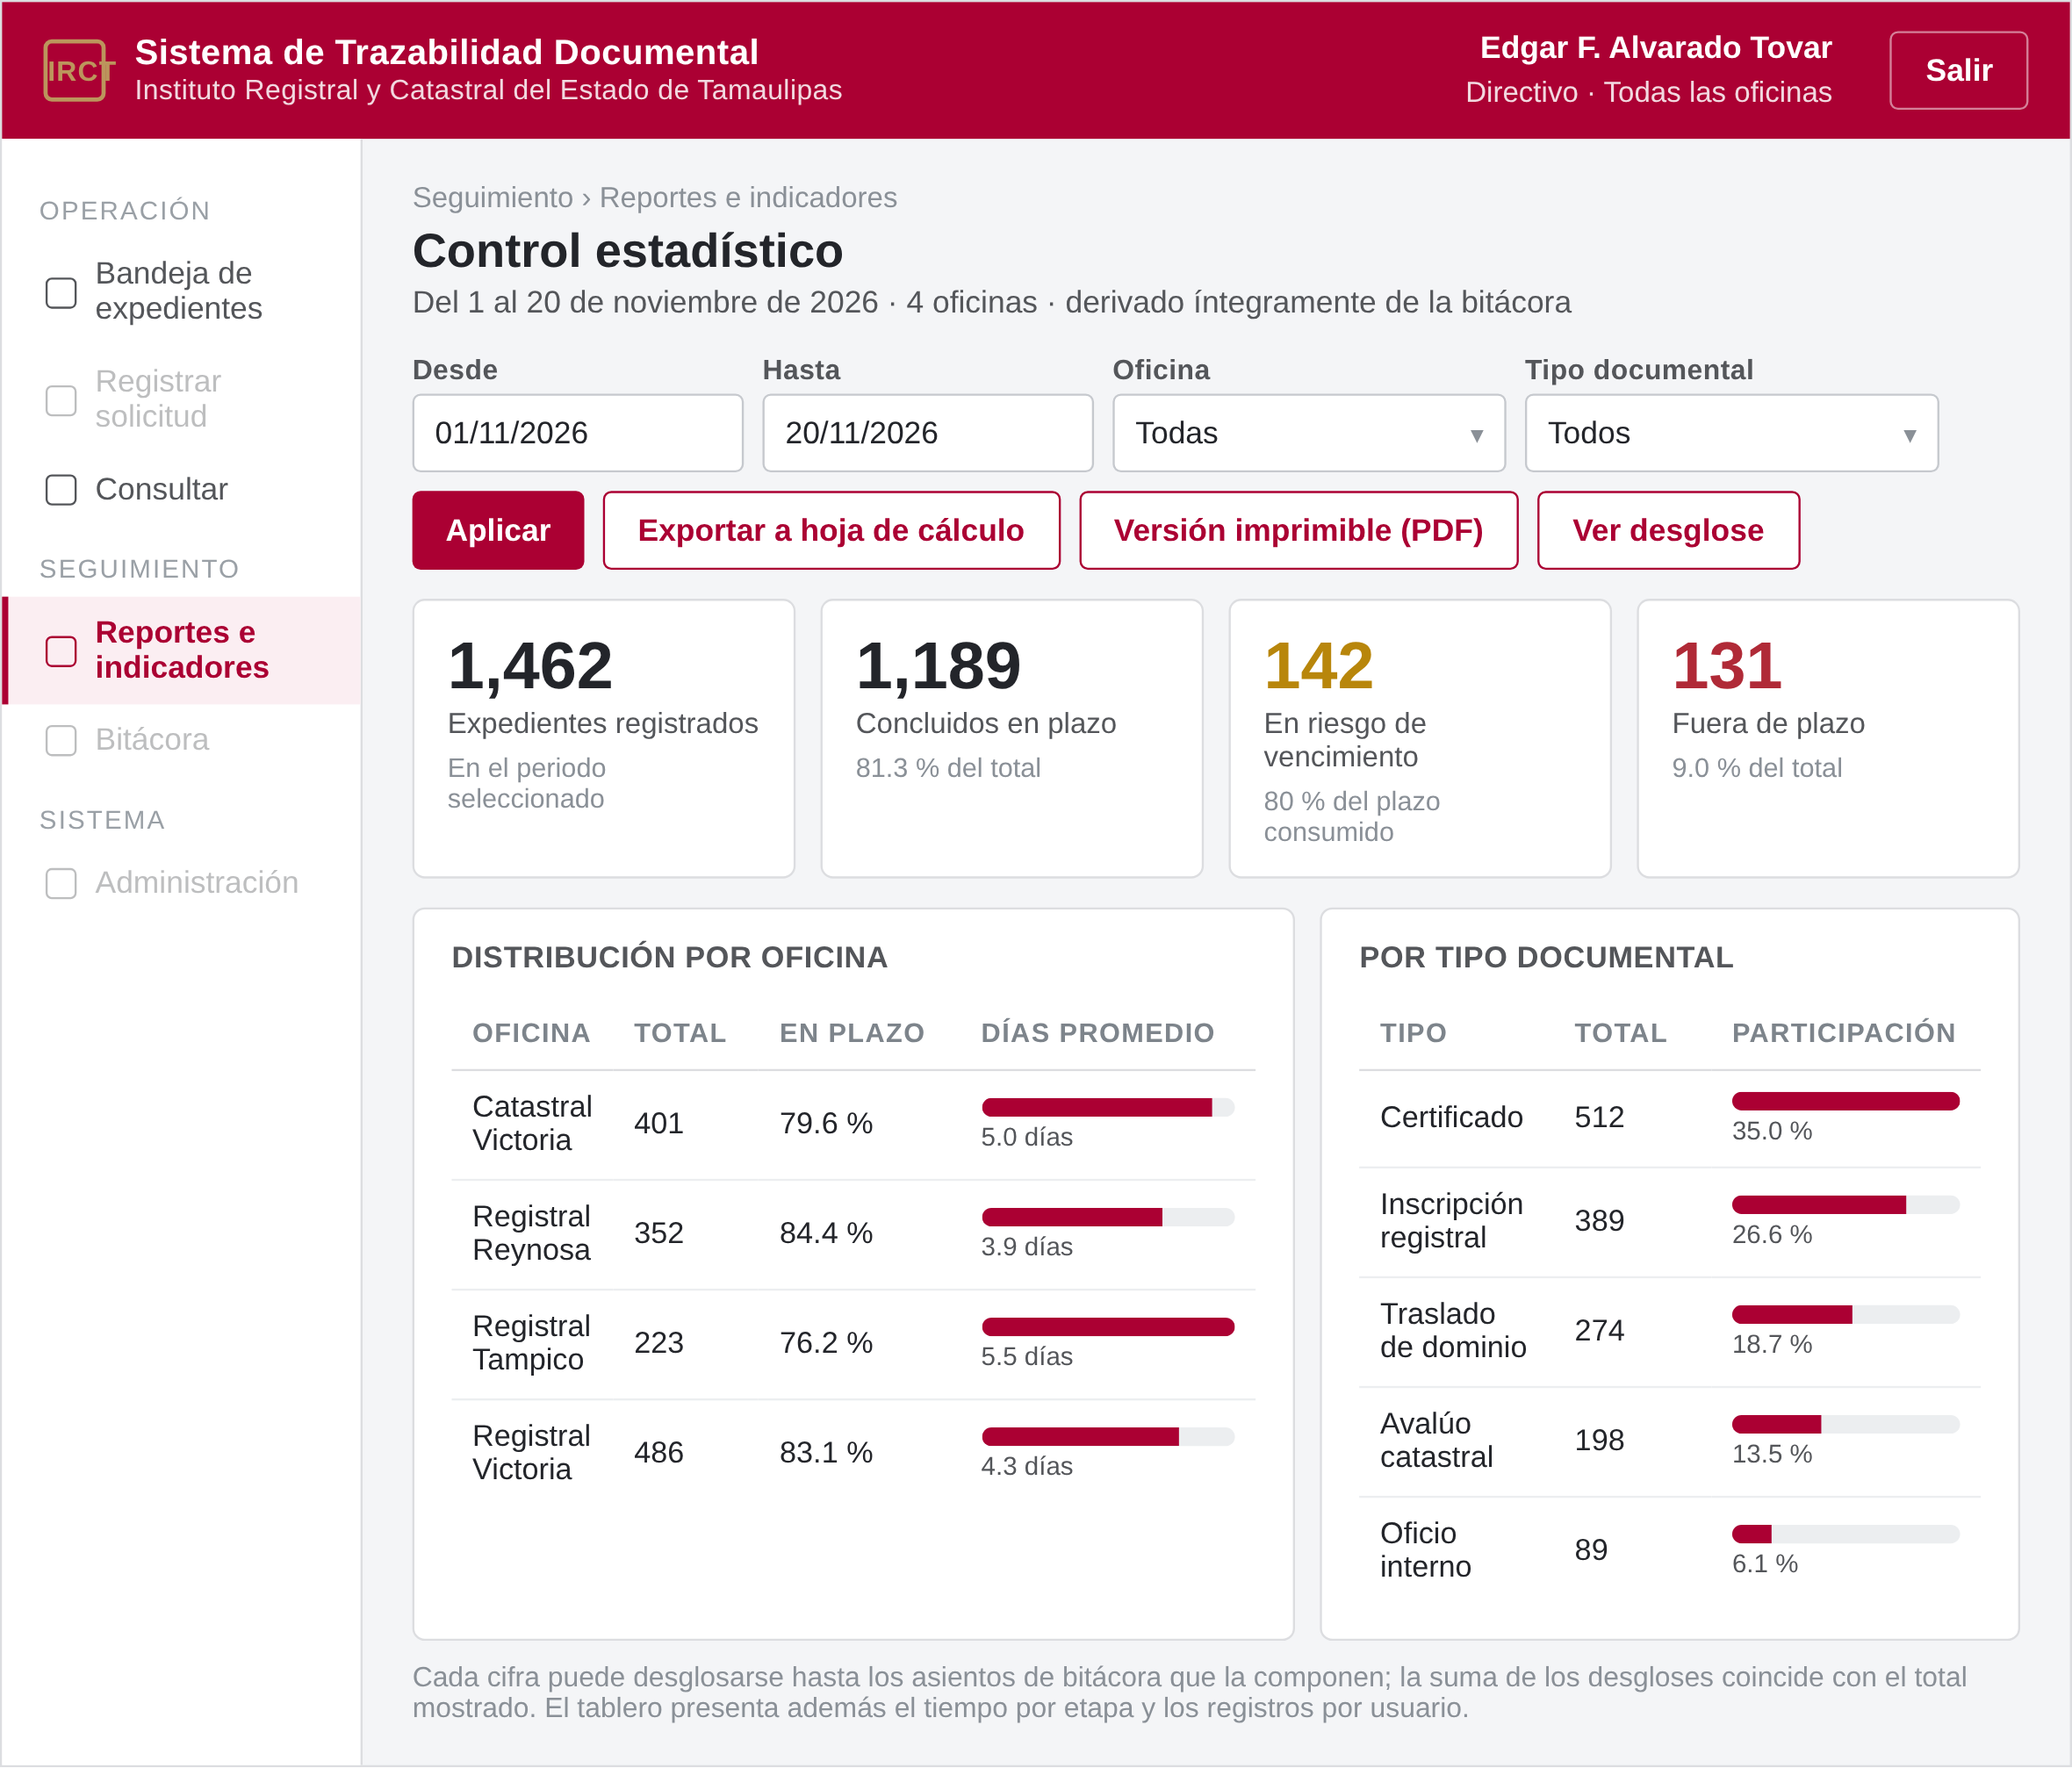
\includegraphics[width=\textwidth,height=0.78\textheight,keepaspectratio]{img/pantalla-tablero.png}
  \caption{Tablero de control estadístico en la sesión de un perfil directivo. Atiende CU-10 y los requerimientos RF-12 y RF-14.}
  \label{fig:pant_estadistico}
\end{figure}

La Figura~\ref{fig:pant_cortes} presenta los dos cortes restantes del mismo tablero. El primero descompone el ciclo en sus cuatro etapas, y es el que vuelve actuable el indicador: un promedio global dice cuánto se tarda, pero no dónde se espera, y de poco sirve acortar el plazo de captura si la demora está en la resolución. Las cuatro etapas son las que los movimientos asentados permiten medir, por la razón que se expone más adelante. La columna de expedientes medidos cumple una función de honestidad estadística: advierte cuántos casos sostienen cada promedio, de modo que una media calculada sobre unos pocos expedientes no se lea como una medición del universo; por la misma razón una etapa sin casos se declara como tal en lugar de promediar cero, que se leería como «se turna el mismo día».

El segundo corte reparte los registros entre los usuarios que los capturaron. Su propósito no es medir a las personas sino detectar la carga desbalanceada entre ventanillas: si una concentra la mitad de los registros de su oficina, el cuello de botella está ahí y no en el plazo del catálogo. Por eso la tabla se limita a los diez primeros y agrupa el resto del padrón en un solo renglón: una lista con todos los nombres invitaría a leerse como una evaluación individual, que no es para lo que se construyó.

\begin{figure}[H]
  \centering
  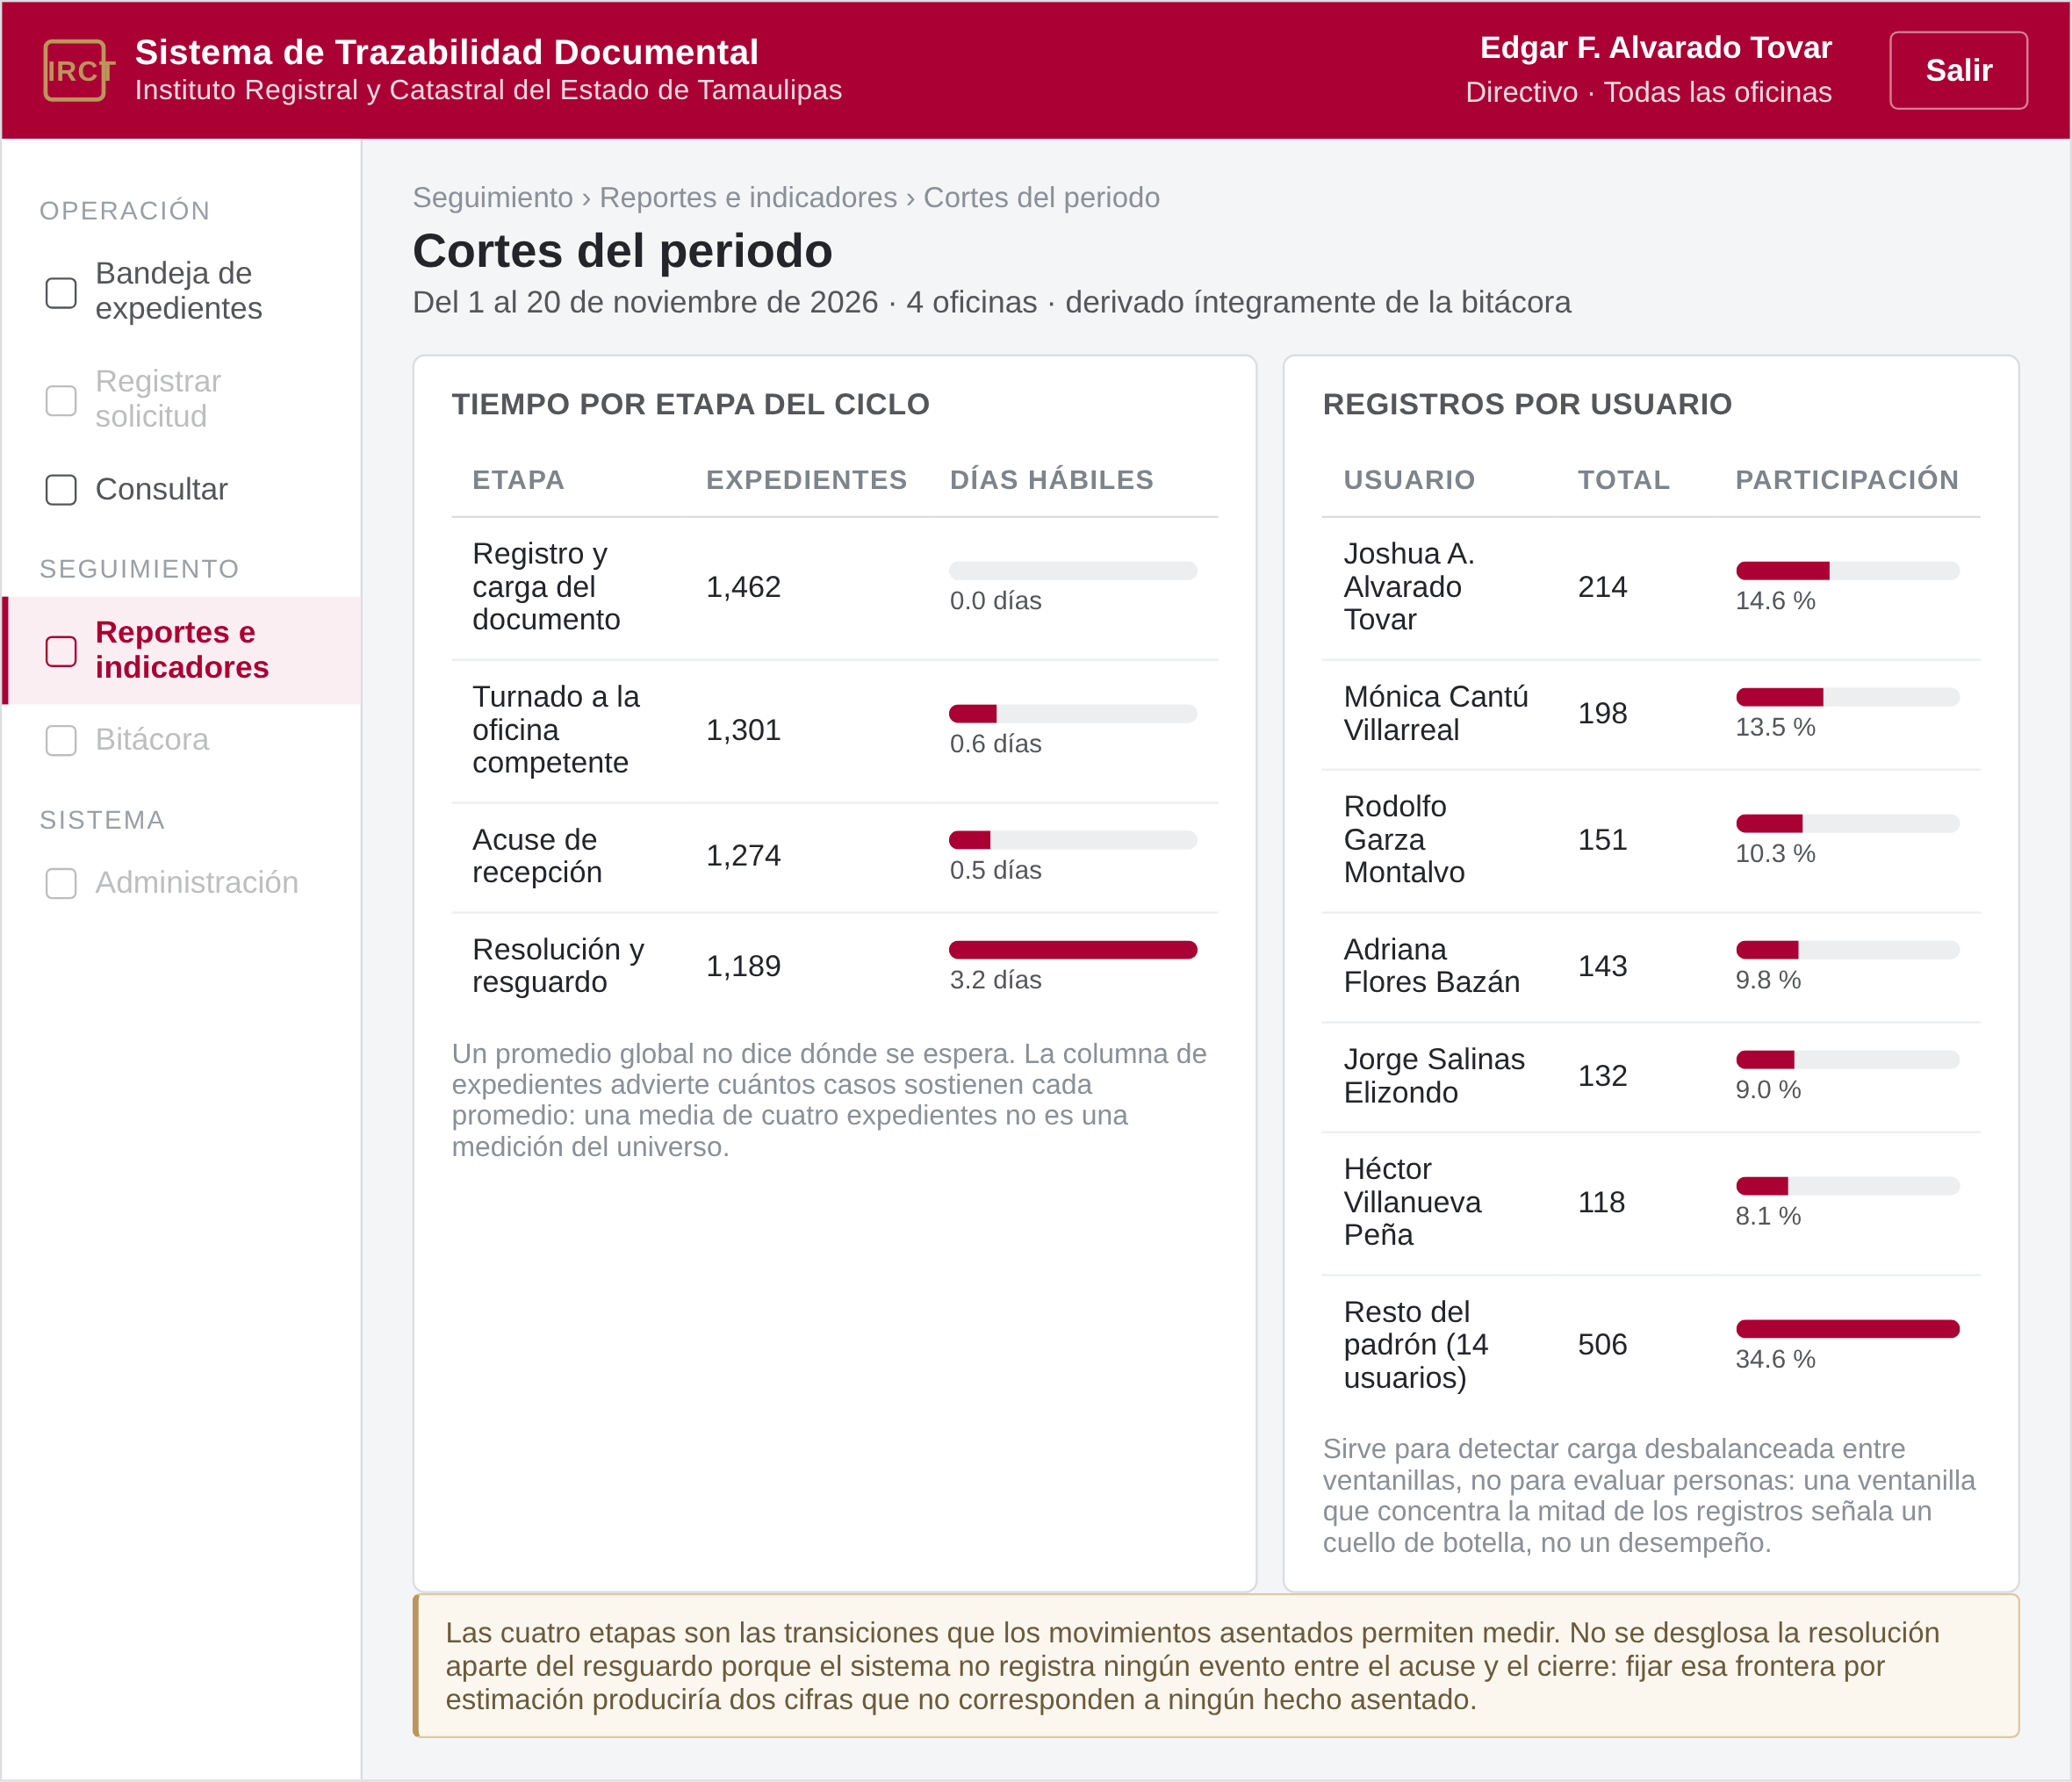
\includegraphics[width=\textwidth,height=0.78\textheight,keepaspectratio]{img/pantalla-cortes.png}
  \caption{Cortes del control estadístico: tiempo medio por etapa del ciclo y distribución de registros por usuario. Atiende CU-10 y el requerimiento RF-12.}
  \label{fig:pant_cortes}
\end{figure}

\subsubsection*{Bitácora institucional}

La Figura~\ref{fig:pant_bitacora} muestra la bitácora, accesible al perfil auditor con alcance institucional y solo de lectura. Cada asiento consigna fecha y hora, usuario, acción, folio y dirección de red de origen. La hora se almacena con precisión de milésima —aunque la pantalla la presente al segundo— porque con precisión de segundo dos asientos simultáneos quedan sin orden y la secuencia de una operación concurrente no podría reconstruirse. El folio se copia en el asiento en lugar de leerse por la llave, de modo que siga siendo legible aunque el expediente se depurara en el futuro: un asiento que depende de otra fila para entenderse no es evidencia. Se asientan tanto las operaciones sobre expedientes como los accesos que no tocan ninguno, como el inicio de sesión o la exportación de un reporte. La nota al pie no describe una intención sino una condición del motor: los privilegios de actualización y borrado están revocados sobre esta tabla para la cuenta con la que la aplicación se conecta, de modo que ningún perfil, incluido el administrador, puede modificar o eliminar un asiento. Es la diferencia entre una bitácora que se promete inalterable y una que lo es.

\begin{figure}[H]
  \centering
  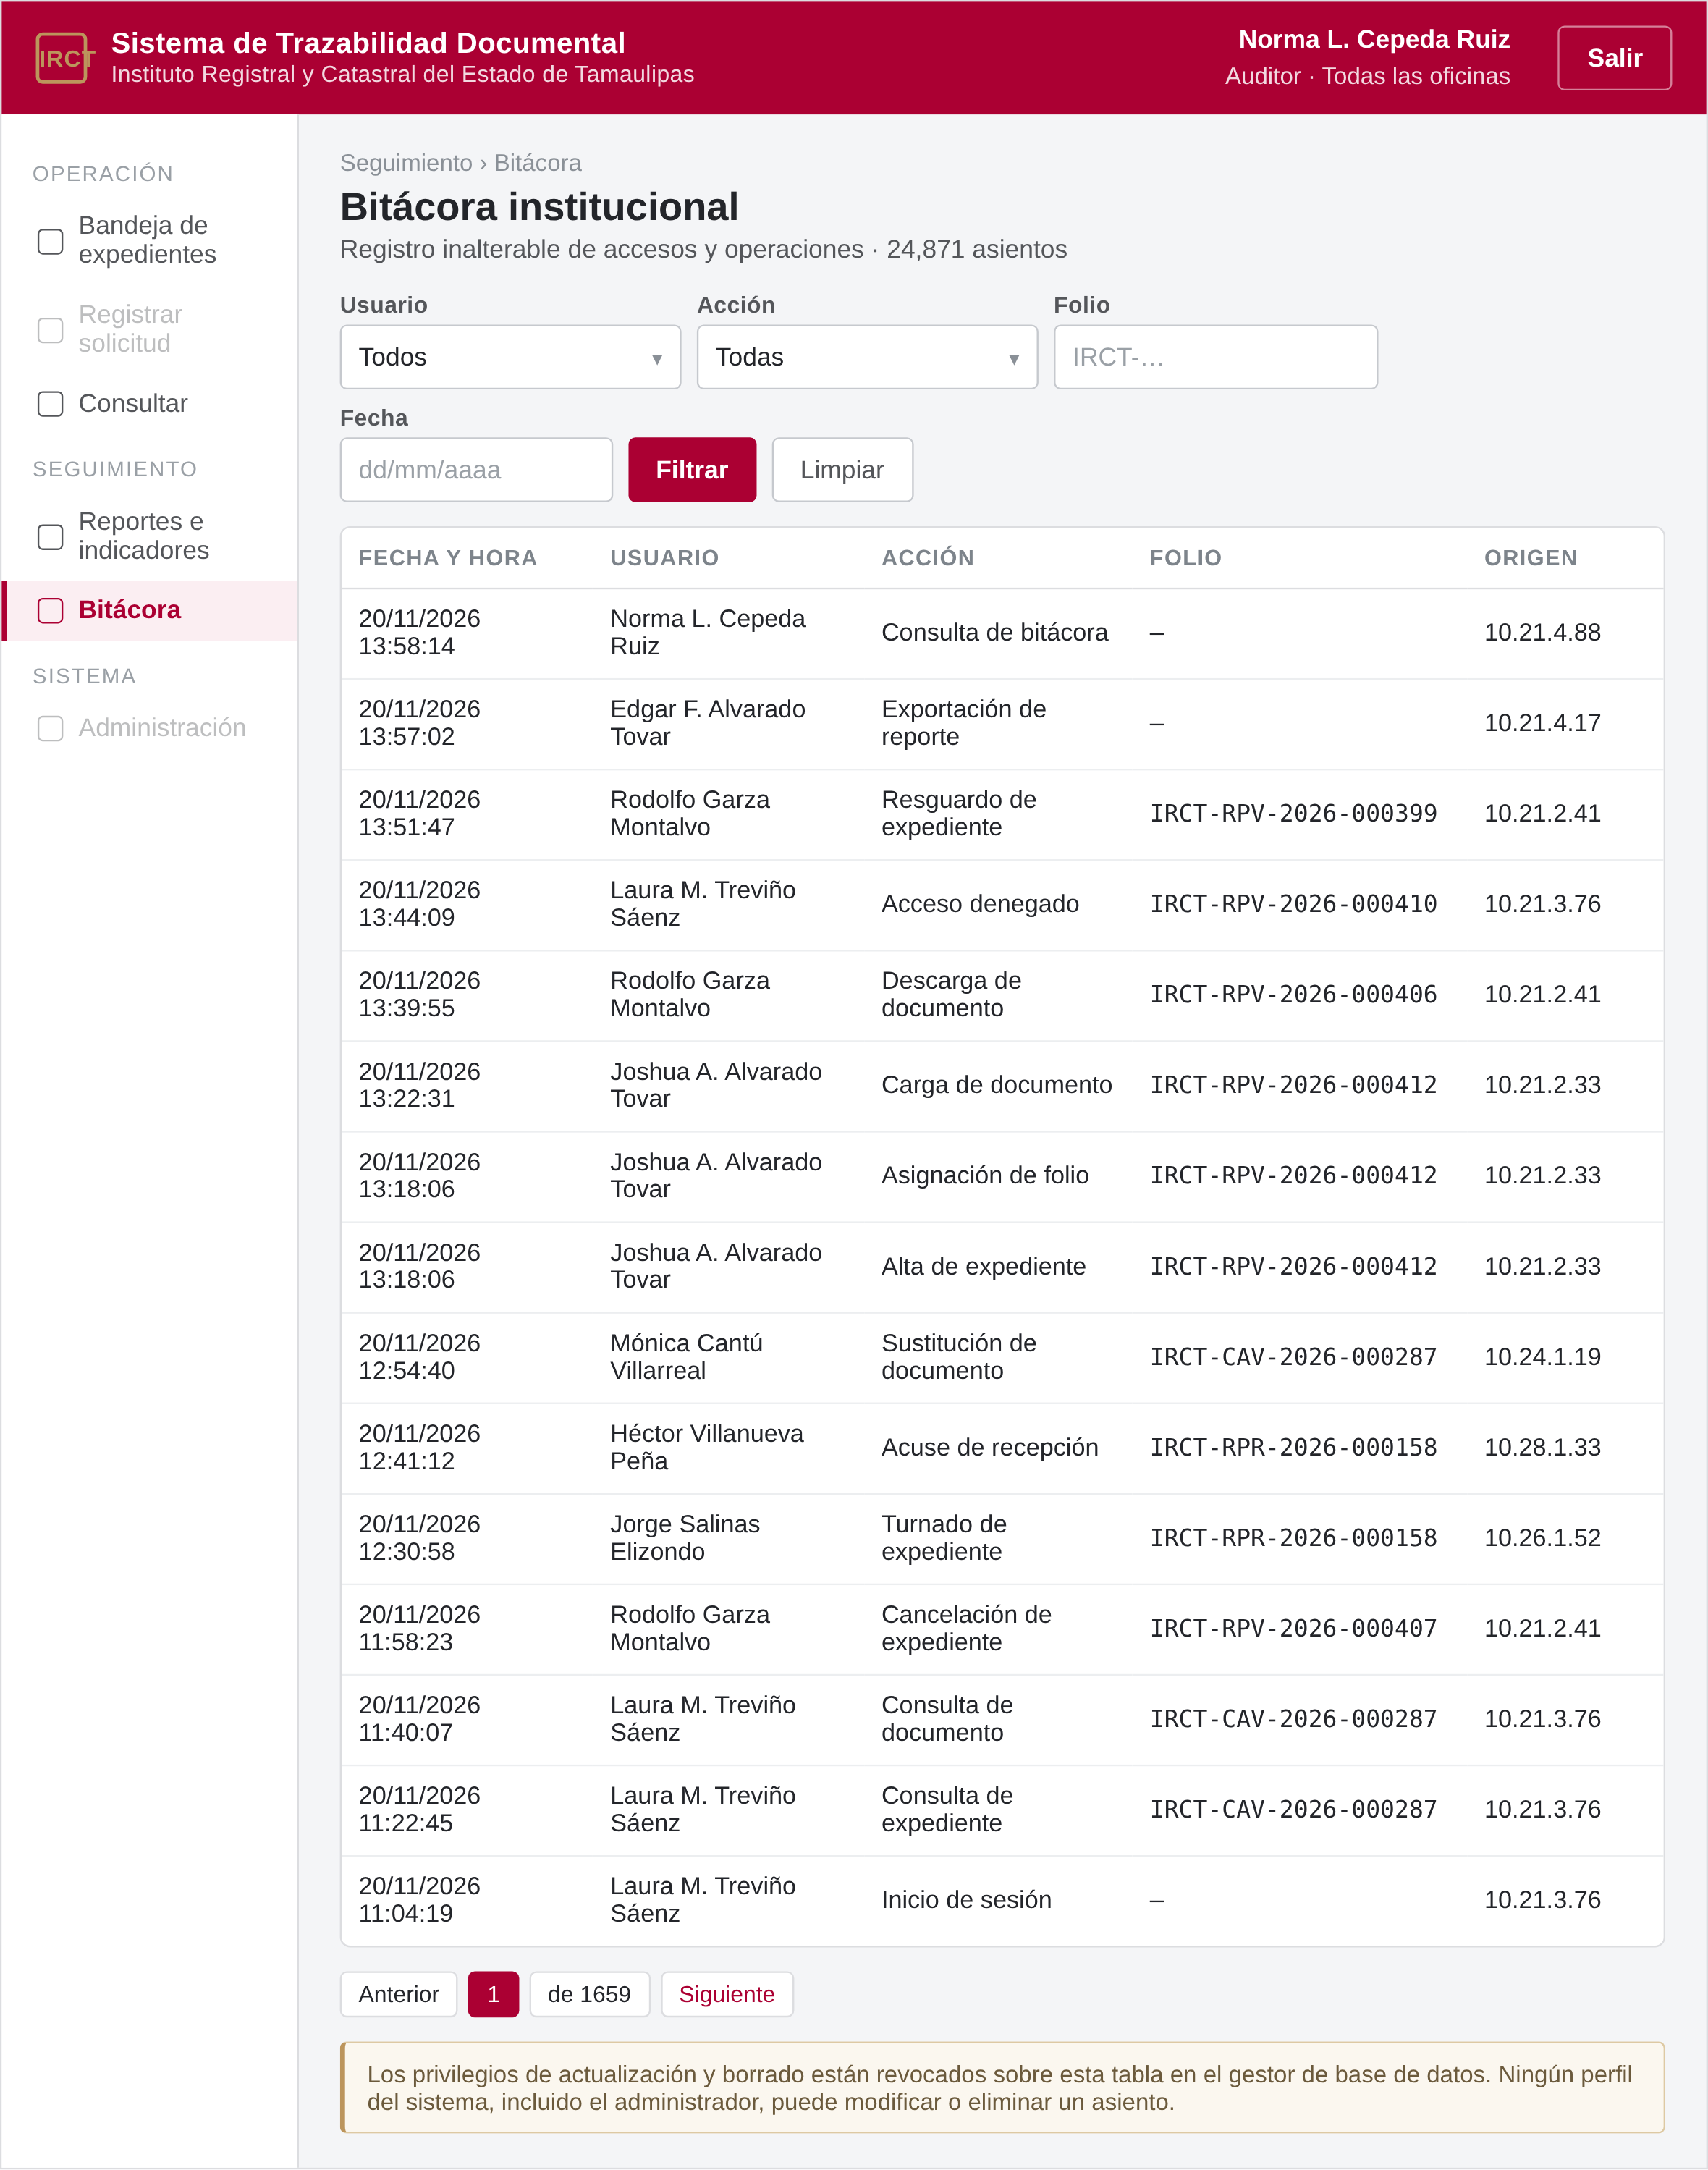
\includegraphics[width=\textwidth,height=0.78\textheight,keepaspectratio]{img/pantalla-bitacora.png}
  \caption{Consulta de la bitácora en la sesión de un perfil auditor. Atiende CU-09 y los requerimientos RF-15 y RF-16.}
  \label{fig:pant_bitacora}
\end{figure}

\subsubsection*{Administración del sistema}

Las dos últimas pantallas corresponden al módulo de administración, que atiende una exigencia explícita del proyecto: que el Instituto pueda administrar usuarios, oficinas, tipos documentales y plazos sin intervención del desarrollador. La razón es práctica antes que técnica. Mientras esas altas se hicieran por sentencias contra la base de datos, el sistema quedaba atado a quien lo construyó, y la primera reforma del reglamento habría obligado a buscar al residente que ya egresó. De poco sirve una solución cuya configuración siga dependiendo de quien la escribió.

La Figura~\ref{fig:pant_usuarios} muestra la administración del padrón. Cada cuenta se compone de un perfil, que decide qué puede hacer, y una oficina de adscripción, que decide sobre qué; un perfil de ámbito de oficina sin oficina se rechaza, porque el alcance global no tendría contra qué filtrar y la persona entraría a un sistema en blanco. La columna de estado distingue tres situaciones que conviene no confundir: activa, bloqueada por intentos fallidos —que se libera sin tocar la contraseña— y dada de baja. La baja es lógica y nunca un borrado, conforme a RF-18: los asientos históricos deben seguir atribuyendo a esa persona lo que hizo mientras estuvo activa, y un borrado los dejaría apuntando a una fila inexistente. El administrador no puede consultar la contraseña de nadie, solo establecerla de nuevo, ni darse de baja a sí mismo. La figura muestra el listado y sus filtros; el formulario de alta y edición ocupa la parte inferior de la misma pantalla y su estructura es la del formulario de la figura siguiente.

\begin{figure}[H]
  \centering
  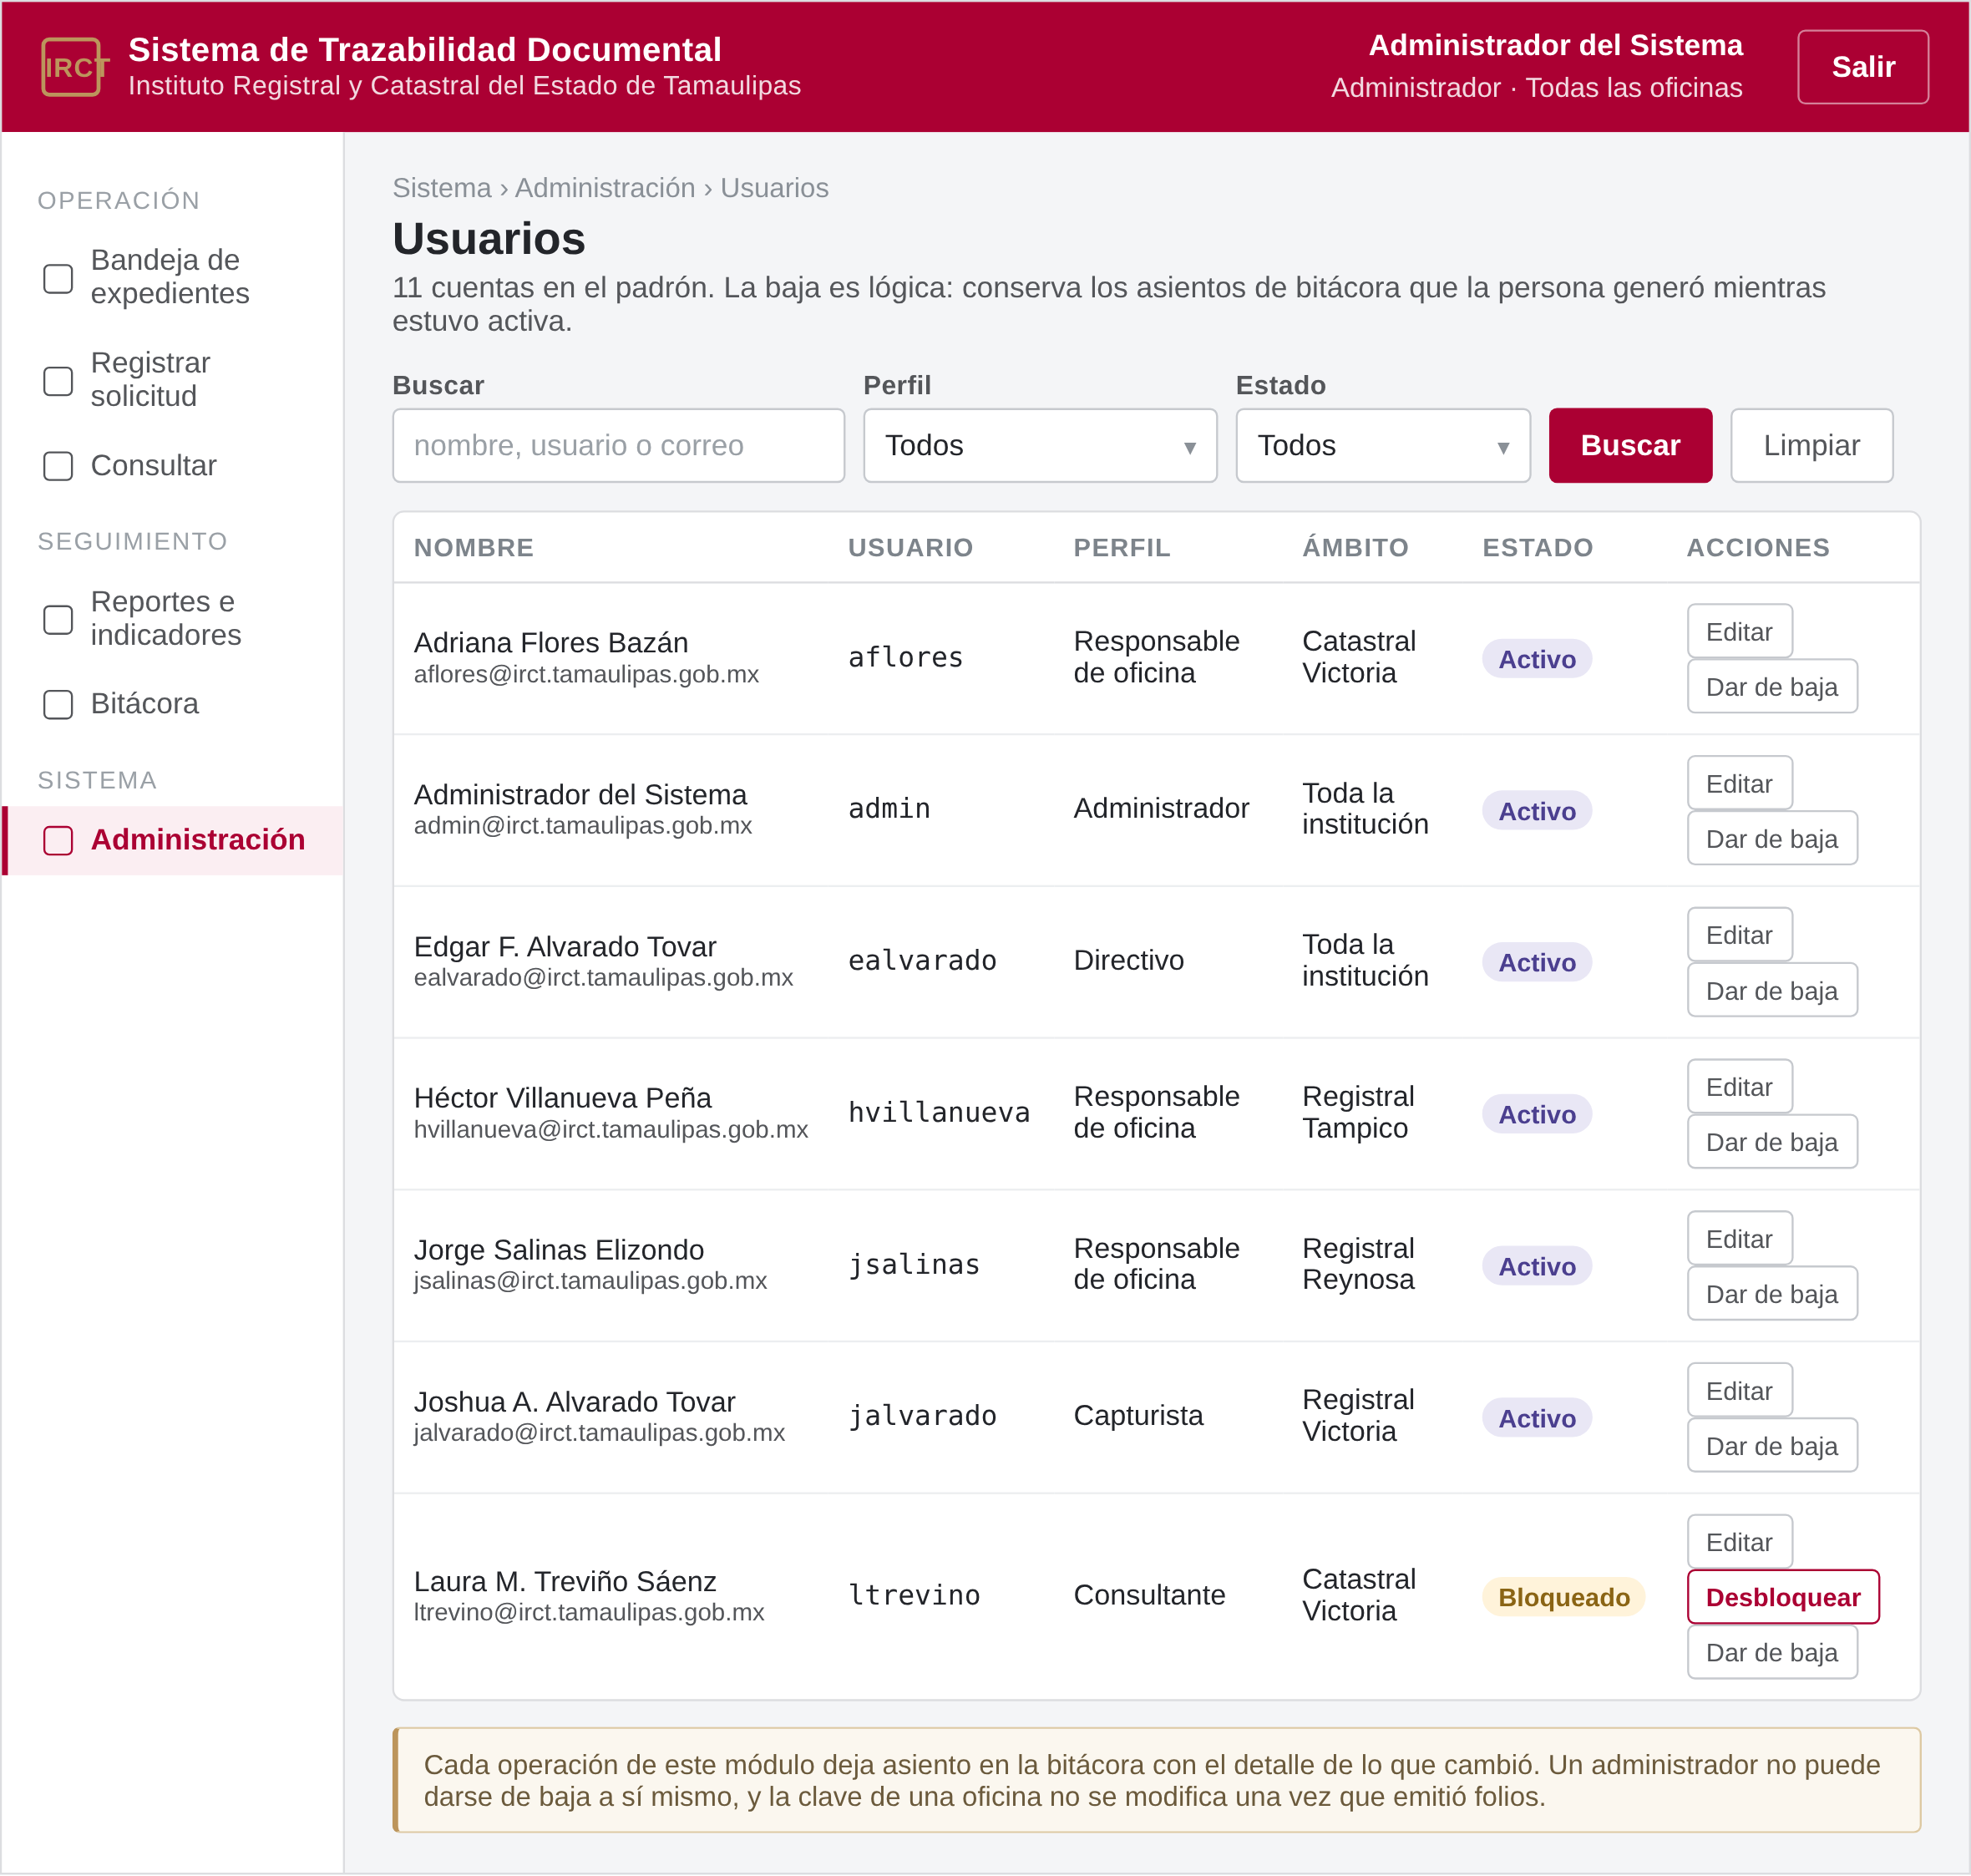
\includegraphics[width=\textwidth,height=0.78\textheight,keepaspectratio]{img/pantalla-usuarios.png}
  \caption{Administración del padrón de usuarios en la sesión del perfil administrador. Atiende CU-11 y los requerimientos RF-17 y RF-18.}
  \label{fig:pant_usuarios}
\end{figure}

La Figura~\ref{fig:pant_catalogo} muestra la edición del catálogo de tipos documentales, que es donde el requerimiento se verifica con más claridad. Agregar un metadato obligatorio o cambiar el plazo de atención es aquí una operación de configuración: el formulario de registro, las reglas de validación, los mensajes de error y el cómputo de la fecha de vencimiento se derivan de este catálogo y aparecen solos, sin tocar una línea de código. Dos salvaguardas acompañan a esa libertad. La primera es que la clave del tipo no se modifica una vez creada, por la misma razón que no se modifica la clave de una oficina: identifica al tipo en los expedientes ya registrados. La segunda es que cambiar el plazo o el conjunto de metadatos sube la versión del catálogo, mientras una corrección de redacción del nombre no la sube; los expedientes ya registrados conservan la versión con la que nacieron y su fecha de vencimiento no se recalcula. Sin esa segunda salvaguarda, una actualización de catálogo haría aparecer como vencidos expedientes que se atendieron en tiempo, y el histórico del tablero cambiaría de forma retroactiva.

\begin{figure}[H]
  \centering
  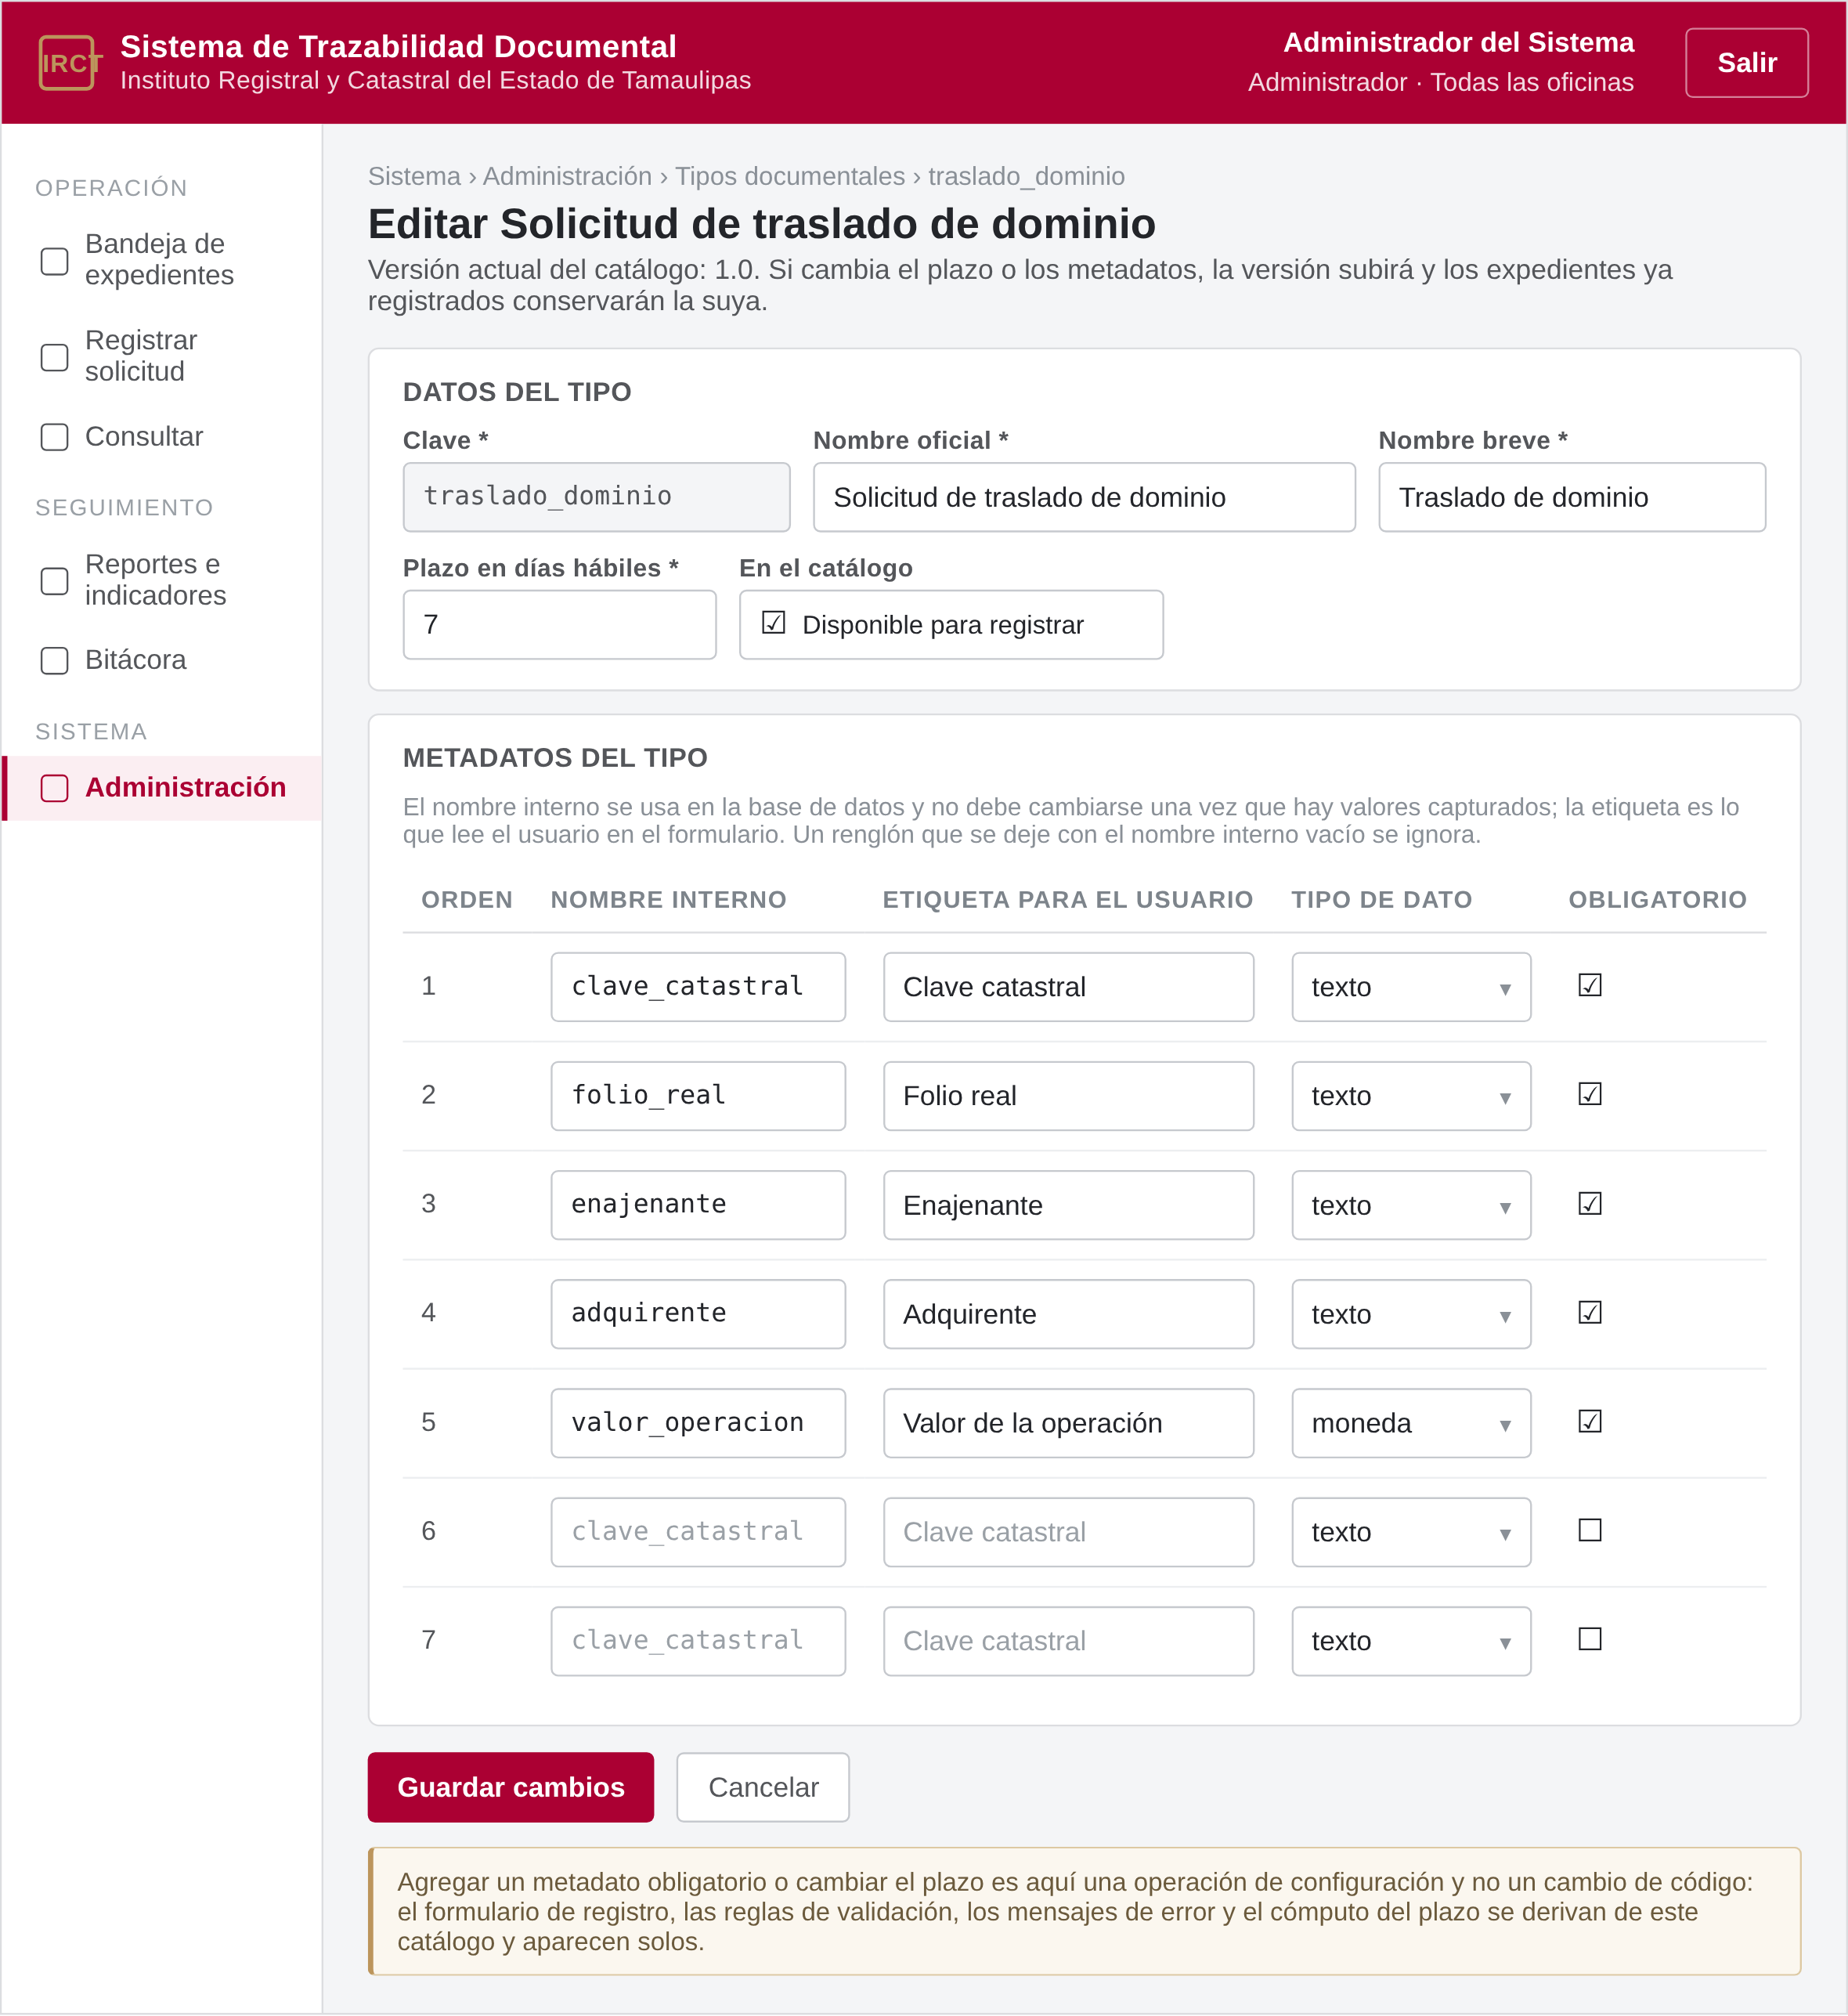
\includegraphics[width=\textwidth,height=0.78\textheight,keepaspectratio]{img/pantalla-catalogo.png}
  \caption{Edición de un tipo documental, con su plazo y sus metadatos obligatorios, en la sesión del perfil administrador. Atiende CU-11 y el requerimiento RF-17.}
  \label{fig:pant_catalogo}
\end{figure}

\subsubsection*{Verificación del sistema}

Las pantallas muestran el sistema funcionando; esta parte expone cómo se comprobó que hace lo que debe. Conviene declarar de entrada el alcance de esa comprobación, porque condiciona la lectura de todo lo que sigue: el sistema se verificó sobre el entorno de desarrollo con datos de prueba, y no en operación con expedientes del Instituto. Su despliegue en la infraestructura institucional excede el periodo de estadía y se enuncia como trabajo futuro en las conclusiones. En consecuencia, aquí no se reportan tiempos de ciclo observados en ventanilla, volúmenes atendidos ni tasas de cumplimiento: reportarlos exigiría una operación que todavía no ha ocurrido, y una cifra sin hecho detrás no es un resultado sino un adorno.

Lo que sí se reporta es reproducible. La verificación descansa en una batería de 127 casos automatizados —72 unitarios y 55 de integración, con 415 aserciones— que se ejecuta con una sola orden contra el mismo gestor del despliegue, MariaDB, y no contra un motor en memoria. Su resultado no depende de quién la ejecute: cualquier lector con el repositorio y Docker puede repetirla y obtener el mismo veredicto. Esa propiedad es deliberada y es el criterio que ordena toda esta sección. Una afirmación sobre el comportamiento de un sistema vale lo que valga la posibilidad de comprobarla, de modo que se prefirió un conjunto de resultados más corto y verificable a uno más vistoso que sólo el autor pudiera atestiguar.

Conviene advertir también qué no se mide y por qué. No se presenta una comparación cuantitativa contra el proceso anterior, pese a ser la cifra que más interesaría, porque el proceso en papel no generaba los registros que permitirían calcularla: no constaba la hora en que un expediente salía de una oficina, ni quién lo consultaba, ni cuánto esperaba antes de ser turnado. Esa imposibilidad es la limitación declarada en la Sección~\ref{subsec:limitaciones}, y es a la vez el hallazgo que motivó el proyecto. El valor del sistema no está en haber reducido una cifra conocida, sino en haber hecho medible lo que antes no lo era.

\paragraph{Cumplimiento de los criterios de aceptación.}
La Tabla~\ref{tab:resultados_criterios} contrasta cada uno de los siete criterios enunciados en la Sección~\ref{sec:propuesta} con la verificación practicada. Cinco quedan comprobados por la batería automatizada. Los dos restantes exigen el sistema desplegado y se declaran pendientes: darlos por cumplidos sin haberlos ejercido afirmaría más de lo que la evidencia sostiene, y un criterio de aceptación que se da por bueno sin ejercerlo deja de ser un criterio.

\begin{table}[H]
  \centering
  \small
  \renewcommand{\arraystretch}{1.3}
  \caption{Verificación de los criterios de aceptación.}
  \label{tab:resultados_criterios}
  \begin{tabularx}{\textwidth}{@{}>{\raggedright\arraybackslash}p{3.2cm}>{\raggedright\arraybackslash}X>{\raggedright\arraybackslash}p{2.0cm}@{}}
    \toprule
    \textbf{Criterio} & \textbf{Verificación practicada} & \textbf{Resultado} \\
    \midrule
    1. Trazabilidad completa & El ciclo completo —alta, carga, turnado, acuse y resguardo— deja sus cinco movimientos asentados, y la prueba reconstruye la secuencia íntegra con usuario, fecha y hora & Verificado \\
    2. Unicidad del folio & Serie de doscientos registros en la misma oficina y año: doscientos folios distintos, secuencia continua y sin huecos. La restricción de unicidad del gestor rechaza además un folio duplicado insertado a propósito & Verificado \\
    3. Inalterabilidad de la bitácora & Intentos de actualización y de borrado de un asiento con la cuenta de la aplicación. El gestor rechaza ambos, y el comando de blindaje lo comprueba en cada arranque & Verificado \\
    4. Indicador y evidencia & Desglose de los indicadores del tablero hasta los asientos que los componen; la suma coincide con el total y ninguna oficina pierde expedientes en el reparto & Verificado \\
    5. Control de acceso efectivo & Acceso a un expediente de otra oficina, por la interfaz y solicitando la dirección del archivo, y descarga sin perfil para ello. Rechazados en las tres vías, con asiento del intento & Verificado \\
    6. Recuperabilidad & El comando de respaldo cubre base y acervo, y el manual técnico documenta la restauración; ejercerla en un entorno limpio requiere la infraestructura del Instituto & Pendiente \\
    7. Apropiación institucional & El módulo de administración permite gestionar usuarios, oficinas, tipos documentales y plazos sin intervención del desarrollador, comprobado por diecisiete casos; la apropiación efectiva exige despliegue y capacitación & Pendiente \\
    \bottomrule
  \end{tabularx}
\end{table}

\paragraph{Cumplimiento de los requerimientos no funcionales.}
La Tabla~\ref{tab:resultados_rnf} contrasta la meta comprometida en la propuesta con el estado de su verificación. Las metas de desempeño bajo carga y las que involucran a personas se distinguen de las demás por una razón de método: dependen del volumen y de los usuarios reales, y ninguno de los dos puede simularse de forma que el resultado signifique algo.

\begin{table}[H]
  \centering
  \small
  \renewcommand{\arraystretch}{1.3}
  \caption{Estado de verificación de los requerimientos no funcionales.}
  \label{tab:resultados_rnf}
  \begin{tabularx}{\textwidth}{@{}>{\raggedright\arraybackslash}p{1.6cm}>{\raggedright\arraybackslash}p{5.2cm}>{\raggedright\arraybackslash}X@{}}
    \toprule
    \textbf{Clave} & \textbf{Meta} & \textbf{Estado de verificación} \\
    \midrule
    RNF-01 & Consulta por folio en menos de 3 s con 50\,000 expedientes y 20 usuarios concurrentes & Pendiente: exige el volumen y la concurrencia reales, que requieren el entorno del Instituto \\
    RNF-02 & Cifrado en tránsito, contraseñas derivadas con sal y revisión contra OWASP & TLS 1.2 y 1.3 configurados en el proxy; contraseñas derivadas con sal, nunca en claro. La revisión formal contra OWASP queda pendiente \\
    RNF-03 & Ningún archivo alcanzable por dirección directa & Verificado: el acervo reside fuera de la raíz pública y la descarga por dirección construida a mano se rechaza \\
    RNF-04 & Respaldo diario con restauración probada & El respaldo de base y acervo está implementado y programado; la restauración queda pendiente de ejercer \\
    RNF-05 & Registro completo en no más de 8 campos y 3 pantallas, tras 30 min de capacitación & Verificado en cuanto a campos y pantallas; el tiempo de captura por personal de ventanilla queda pendiente de medir \\
    RNF-06 & Interfaz responsiva desde 1\,024 px en los navegadores del Instituto & Implementada desde 1\,024 px; la comprobación en los equipos del Instituto queda pendiente \\
    RNF-07 & Código versionado y manual técnico de despliegue & Verificado: código en repositorio propio y manual técnico de 36 páginas entregado \\
    RNF-08 & Despliegue por contenedores, equivalente en local y en el Instituto & Verificado en el entorno de desarrollo con una sola orden; la equivalencia con el entorno del Instituto queda pendiente \\
    \bottomrule
  \end{tabularx}
\end{table}

\paragraph{Tiempos del ciclo documental.}
El tablero descompone el ciclo en cuatro etapas —registro y carga del documento, turnado a la oficina competente, acuse de recepción, y resolución y resguardo—, que son las cuatro transiciones que los movimientos asentados permiten medir. No se desglosa la resolución aparte del resguardo porque el sistema no registra ningún evento entre el acuse y el cierre, y fijar esa frontera por estimación produciría dos cifras que no corresponden a ningún hecho asentado. El cómputo se practica en días hábiles, con la misma definición que fija la fecha de vencimiento, y su corrección está comprobada por prueba automatizada: lo verificado es el mecanismo de medición, no una medición. Las cifras que arroje existirán cuando el sistema opere con expedientes reales, y es entonces cuando la reducción del tiempo de ciclo —el tercer propósito del objetivo general— podrá darse por demostrada.

Dos decisiones de ese cálculo merecen nota, porque atienden al mismo criterio que ordena esta sección. La primera es que el tablero declara junto a cada promedio cuántos expedientes lo sostienen, de modo que una media calculada sobre unos pocos casos no se lea como una medición del universo. La segunda es que una etapa sin casos se declara como tal en lugar de promediar cero, que se leería como «se turna el mismo día». Un indicador que no distingue entre «no hay demora» y «no hay datos» induce exactamente el error que el control estadístico debía evitar.
